\section{State Redistribution }\label{sec:srdAlg}

We first describe the second order accurate version of the State
Redistribution Algorithm. 
This helps simplify the notation and make the
algorithm more intuitive.   
At several places there are choices
to make, and we discuss the alternatives and the reason behind our
choices.  
Section \ref{sec:ho} presents the higher order version of the algorithm in full generality.

\subsection{State Redistribution Preprocessing}

To start, we define a number of quantities associated with each cell of the mesh:

\begin{itemize}
\item
{\bf Each cut cell finds adjacent cells to {\em temporarily} merge with.}

\vspace*{.1in}
For each cut cell in the mesh, find  one or more neighbors until the
volume of the temporarily merged cell is at least half the area of an uncut cell, i.e., 
\begin{equation} \label{eqn:vmerge}
\sum_{k \in M_{i,j}} V_{k} \geq \frac{1}{2}\Delta x\Delta y,
\end{equation}
where $M_{i,j}$ denotes the set of cell indices that belong to merging neighborhood $(i,j)$.
We call this the 
{\em  merging neighborhood} or {\em merging tile}.  
A small cell can be merged with cells in the direction closest to the 
boundary normal (Figure \ref{fig:neighborhoods}, left), or with all cells 
that are at most e.g. one cell away, that is, cells located on the $3 \times 3$ 
tile centered at the small cell (Figure \ref{fig:neighborhoods}, right).
The larger the neighborhood the more diffusive the results. 
For smooth solutions a $3 \times 3$ is fine, but for shocks this is less so.
Therefore we use the normal neighborhood everywhere possible.

\begin{figure}[t]
    \centering
    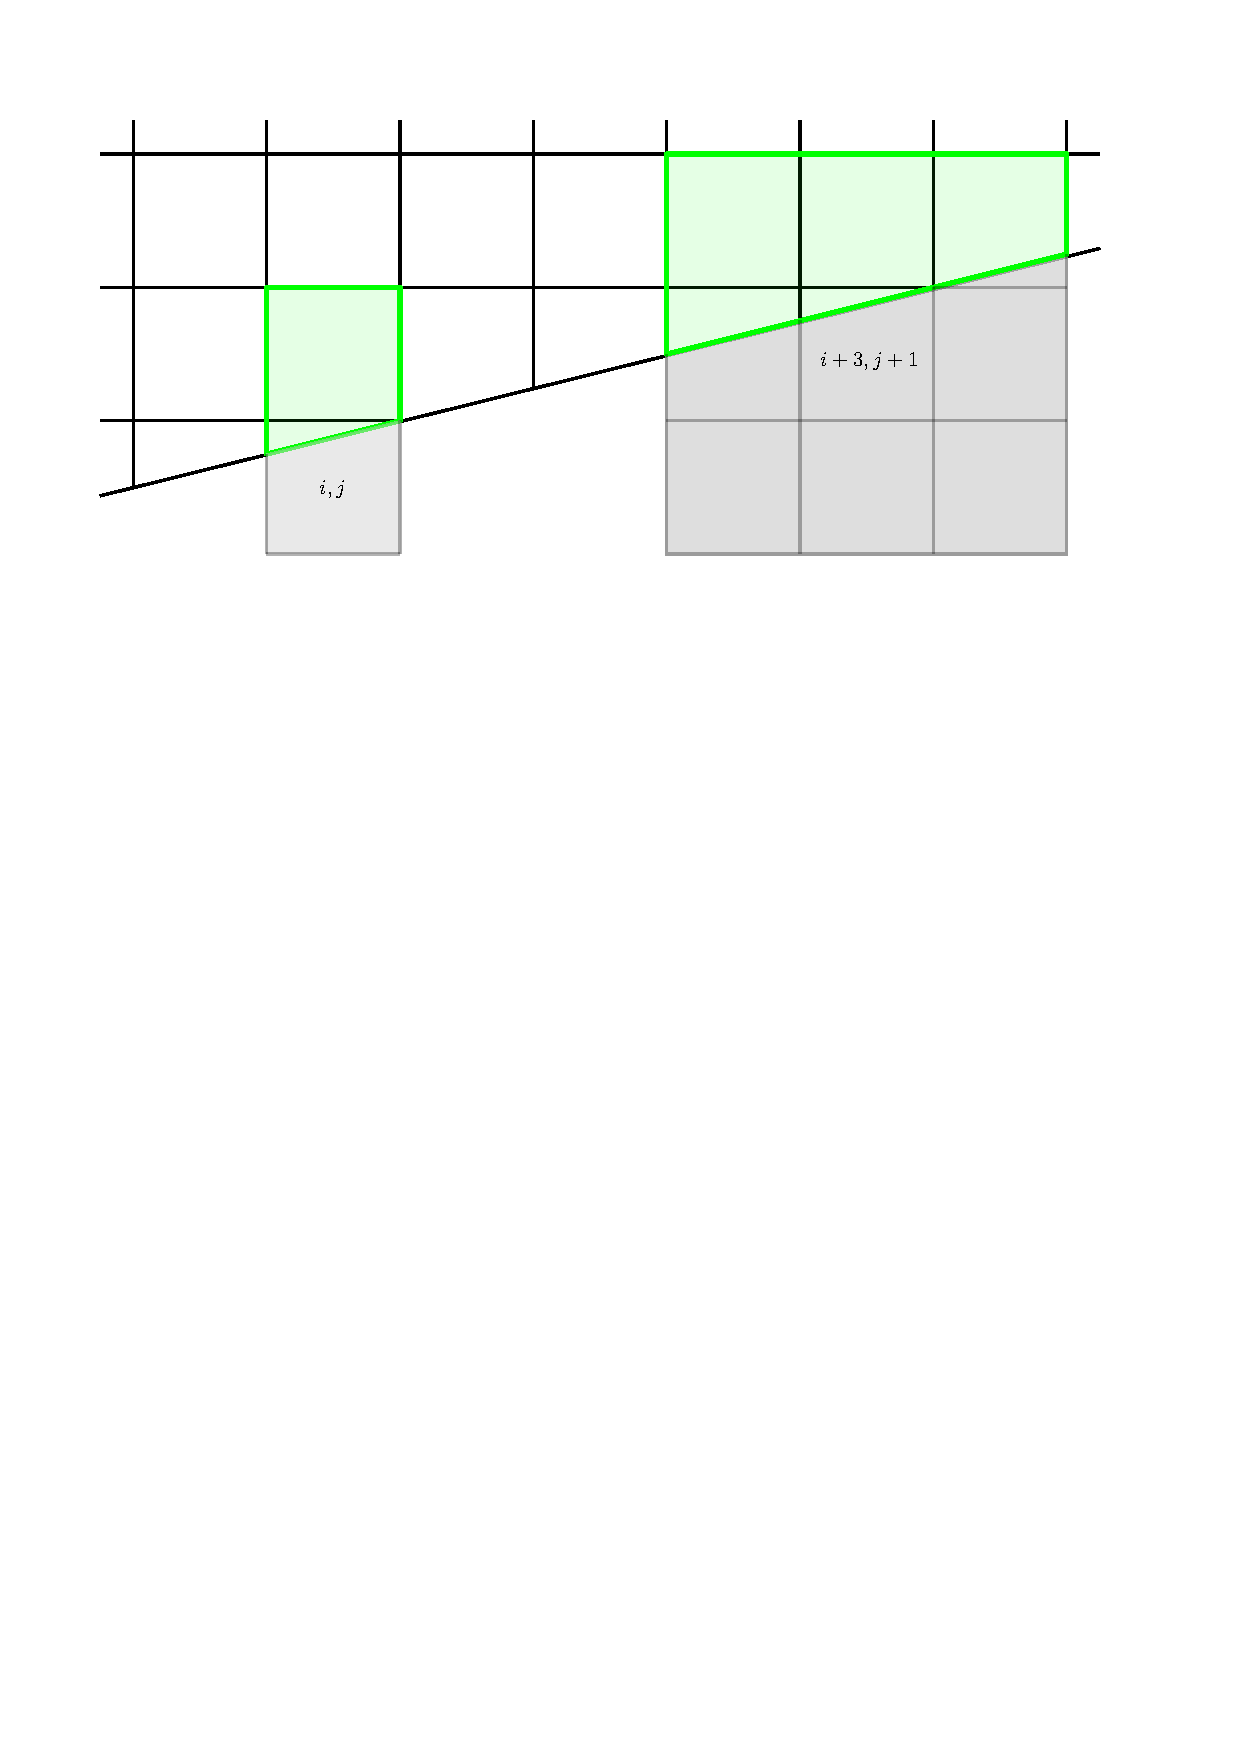
\includegraphics[width=0.5\linewidth]{figs/neighborhoods.pdf}
    \caption{\sf On the left, a small cell is merged with a cell in the direction 
    normal to  the wall.  On the right, a small cell is merged with neighbors that are at most one cell away, i.e., cells located in the $3\times3$ tile.}
    \label{fig:neighborhoods}
\end{figure}


There are instances where the normal neighborhood cannot be used, e.g., if a neighboring cell is also cut and the
merging neighborhood is not sufficiently large (Figure \ref{fig:normalneighborhood}).  In this case, we must merge with cells on the $3\times3$ tile (Figure \ref{fig:3x3neighborhood}), or, if that merging neighborhood is not large enough, with cells on the $5 \times 5$ tile.

\begin{figure}[h]
\hspace*{.5in}
	\subfloat[\sf Normal neighborhood (in red) for both small cells in the right corner.]{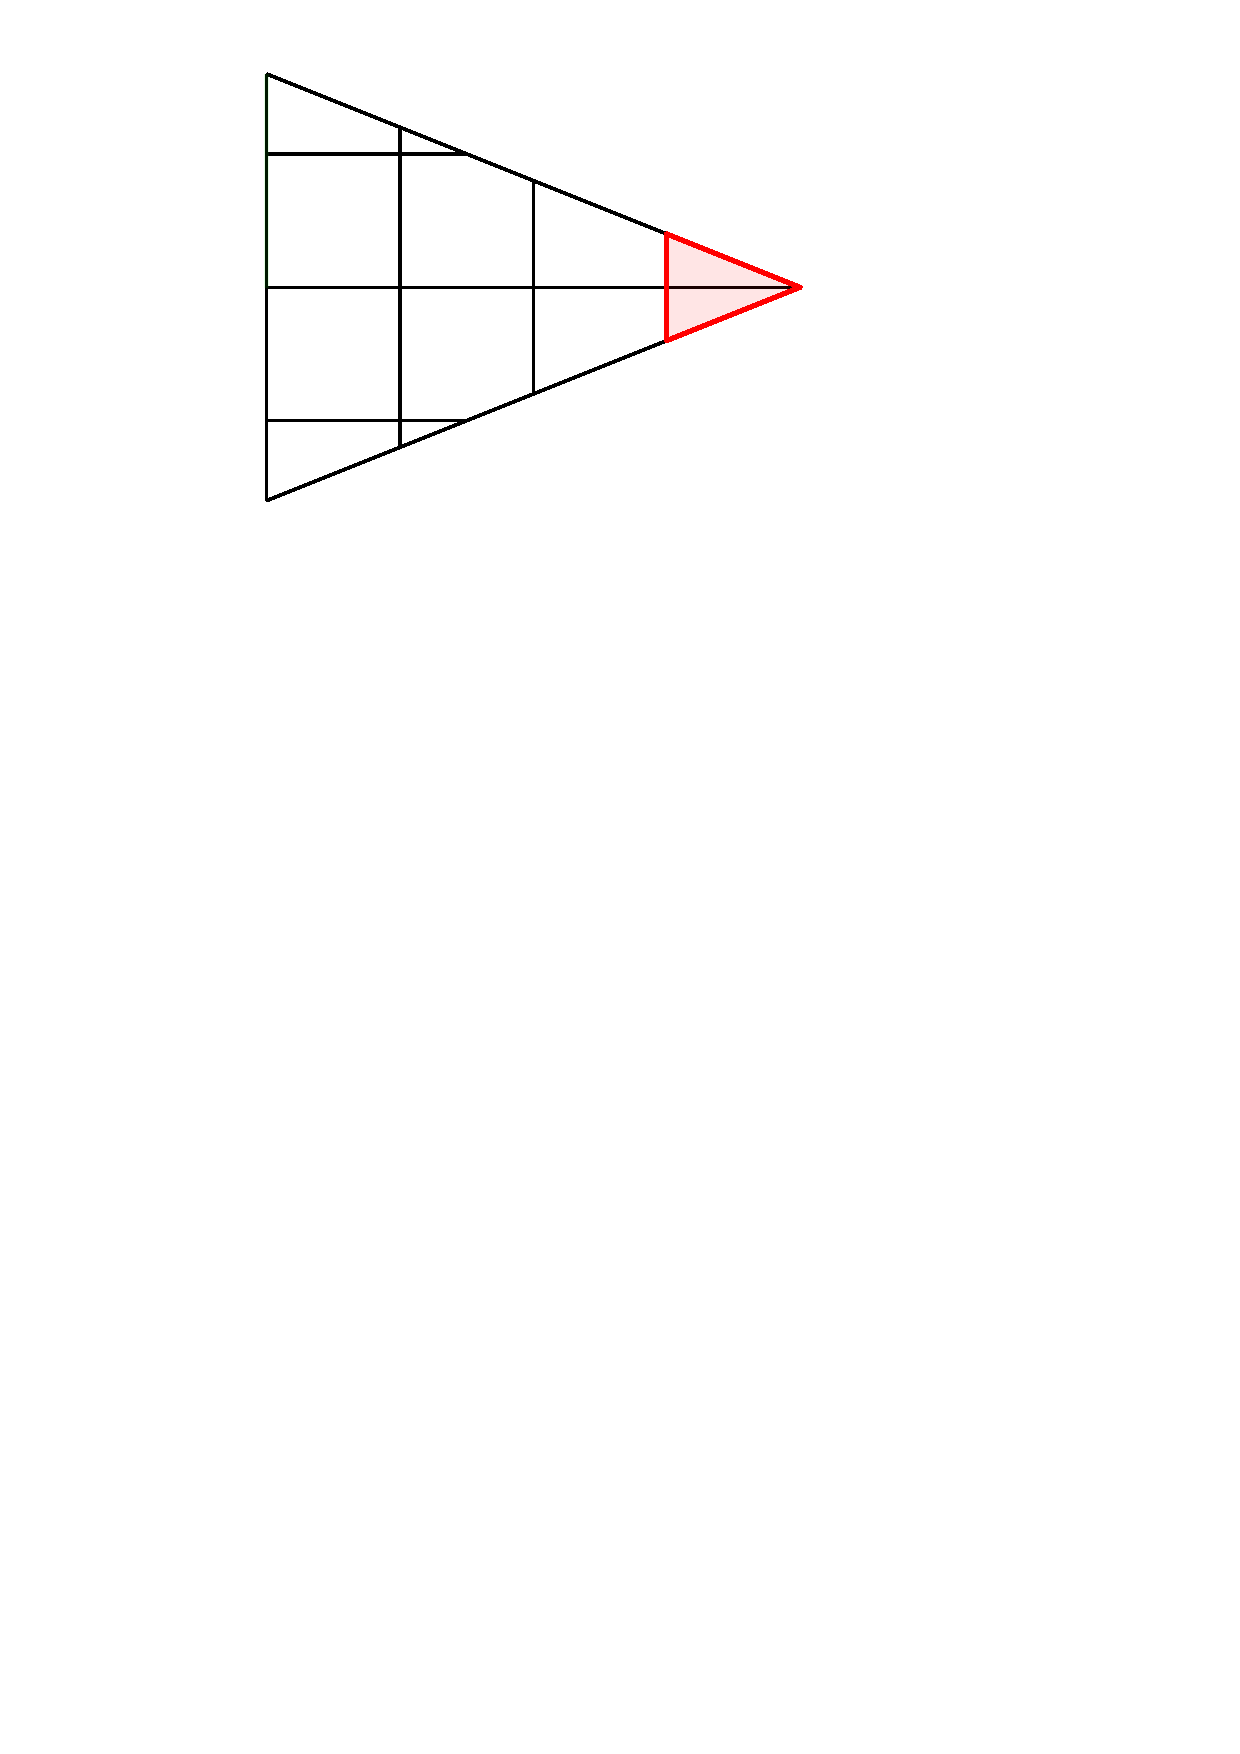
\includegraphics[width=.30\textwidth]{figs/normaldirection1.pdf} \label{fig:normalneighborhood}}
	\hfill
	\subfloat[\sf $3\times 3$ merging neighborhood for both small cells in the right corner.]{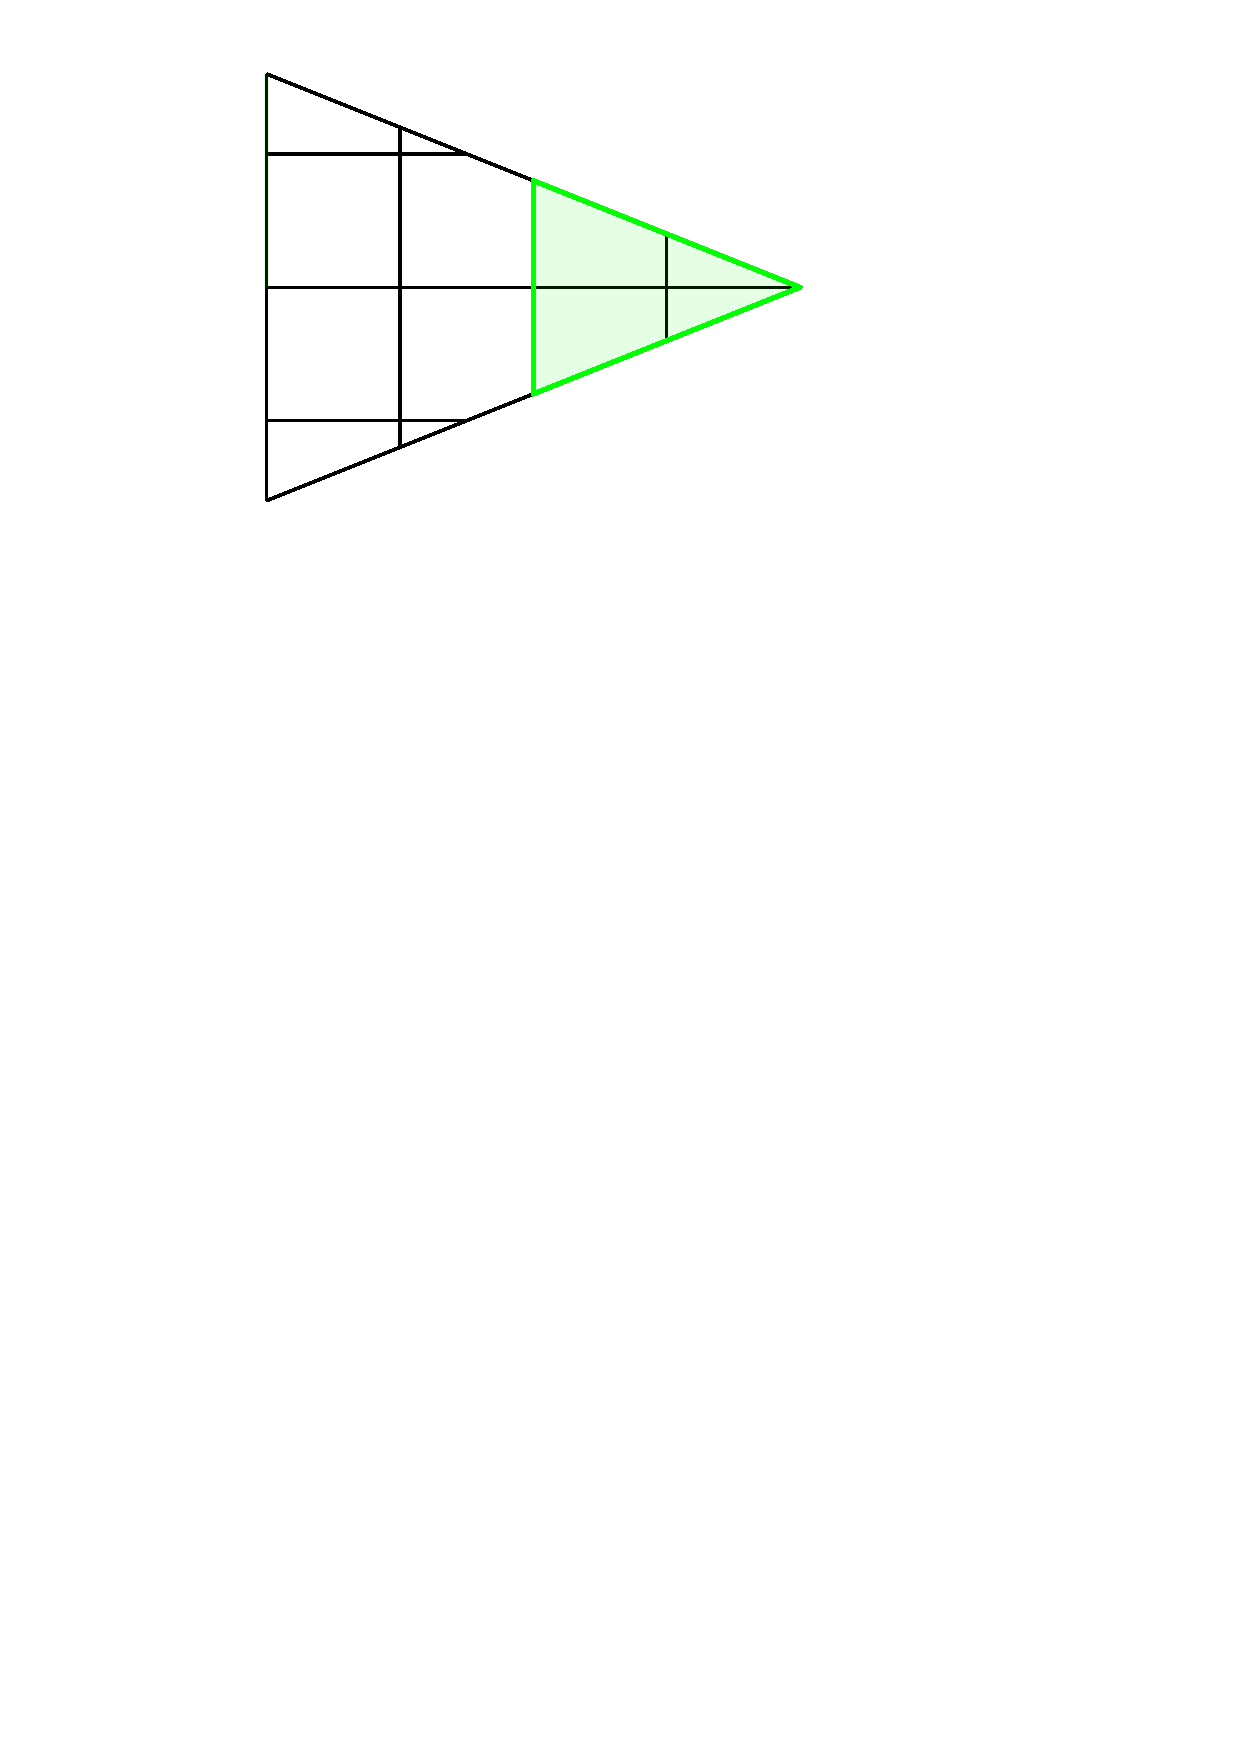
\includegraphics[width=.30\textwidth]{figs/normaldirection2.pdf} \label{fig:3x3neighborhood}}
	\caption{\sf It can happen that merging only in the normal neighborhood is not 
        large enough, e.g. if the small cell merges with another small cell.  
        In this case, we use the $3\times 3$ tile, or $5\times5$ neighborhood 
        until the volume constraint \eqref{eqn:vmerge} is satisfied.}
\end{figure}
% If the neighboring cell 
% is also cut, it can happen that the
% merged cell is not sufficiently large (SHOW EXAMPLE?). 
% Next we try a 2 by 2
% neighborhood, including the original cut cell. Later we also show
% results using a 3 by 3 neighborhoods. However the larger the
% neighborhood the more diffusive the results.

% Note that this does not have the difficulty of cell merging, since 
% overlapping neighborhoods are allowed. 

\item
{\bf Each cell counts how many neighborhoods it is a part of.}

\vspace*{.1in}
A full cell is its own merging neighborhood, since it has sufficient
volume all by itself.
%However, we will still refer to all cells as having a
%merging neighborhood.  
%Figure \ref{fig:overlappingneighs} shows an example of a
%cut cell mesh with all merging neighborhoods plotted.  Also displayed
%are the number of overlapping neighborhoods for each cell. 
%This is what we call the neighborhood {\em count} referred to above.
%\begin{figure}
%	\subfloat[]{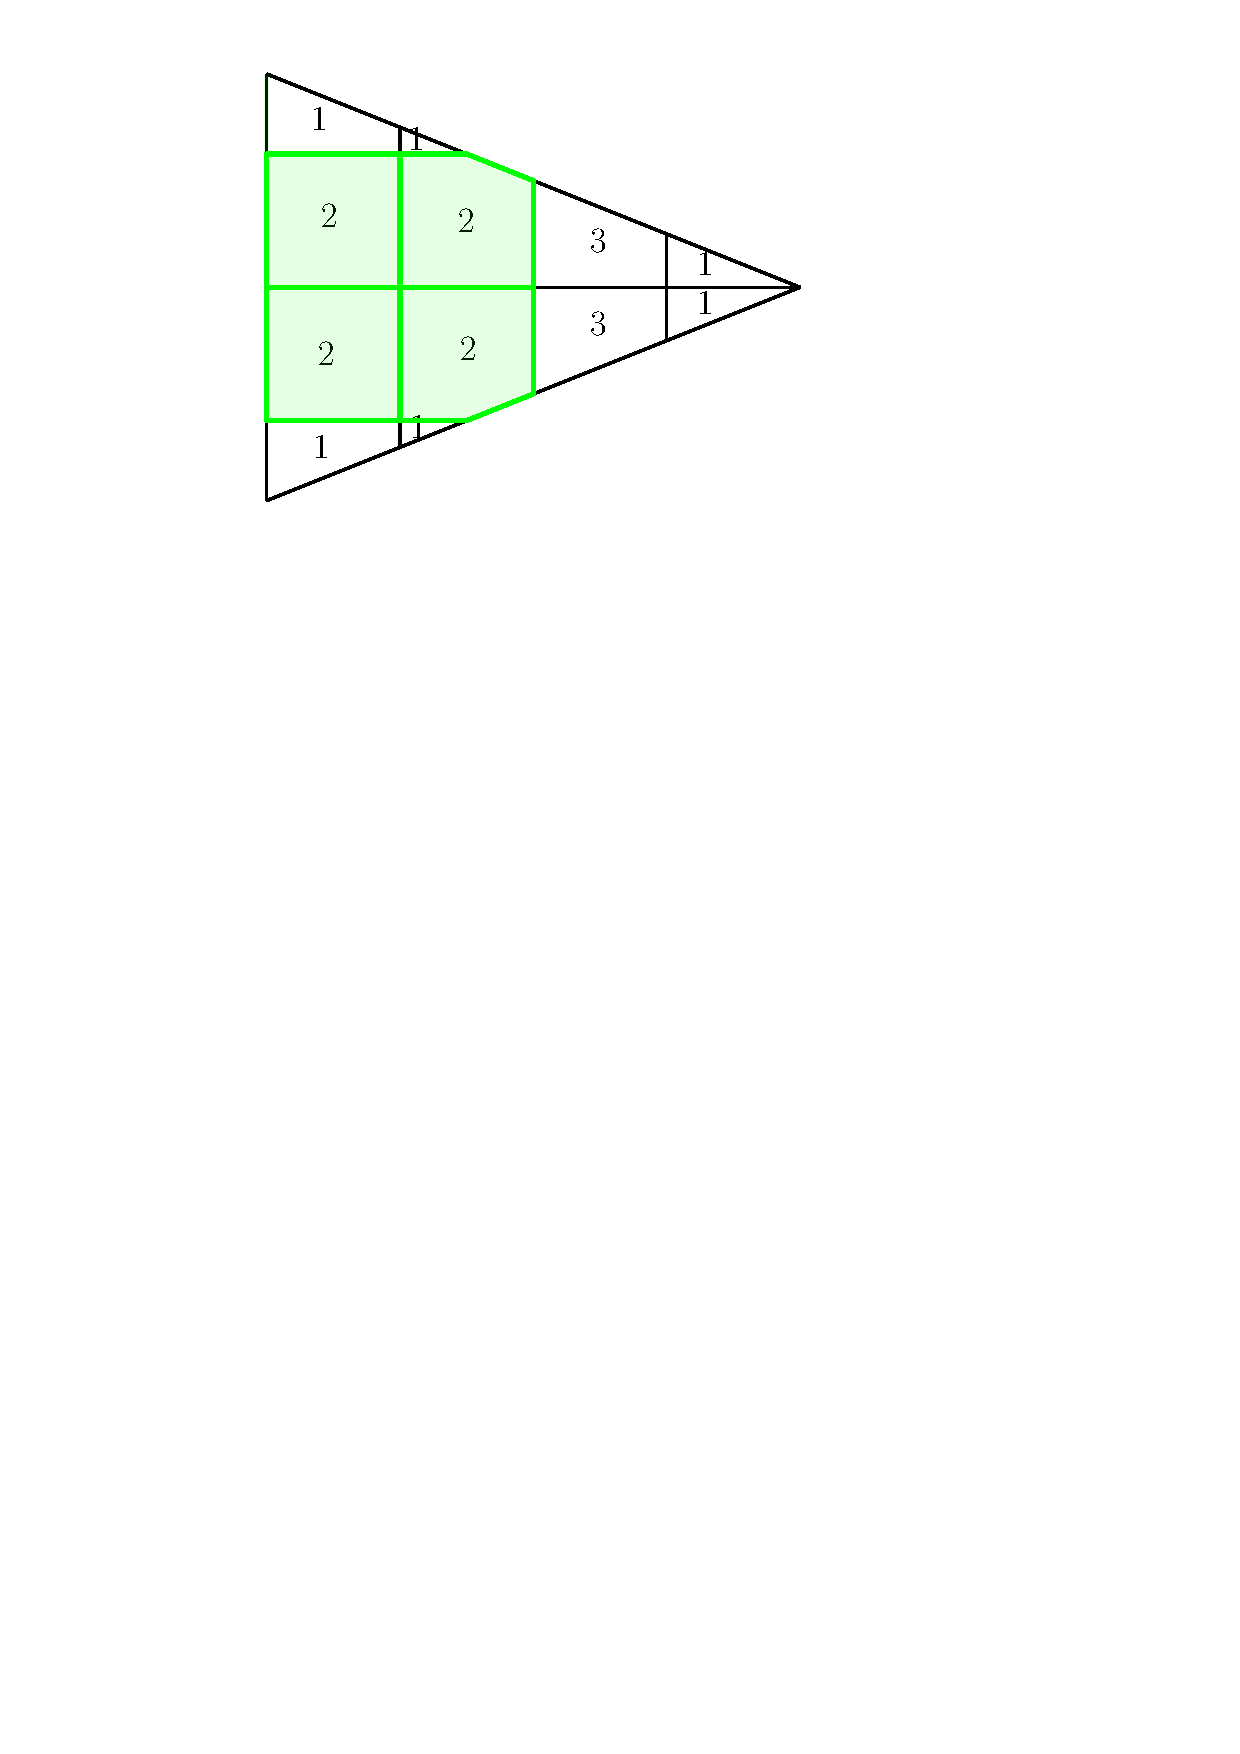
\includegraphics[width=.24\textwidth]{figs/numoverlaps1.pdf} \label{fig:numoverlaps1}}
%	\hfill
%	\subfloat[]{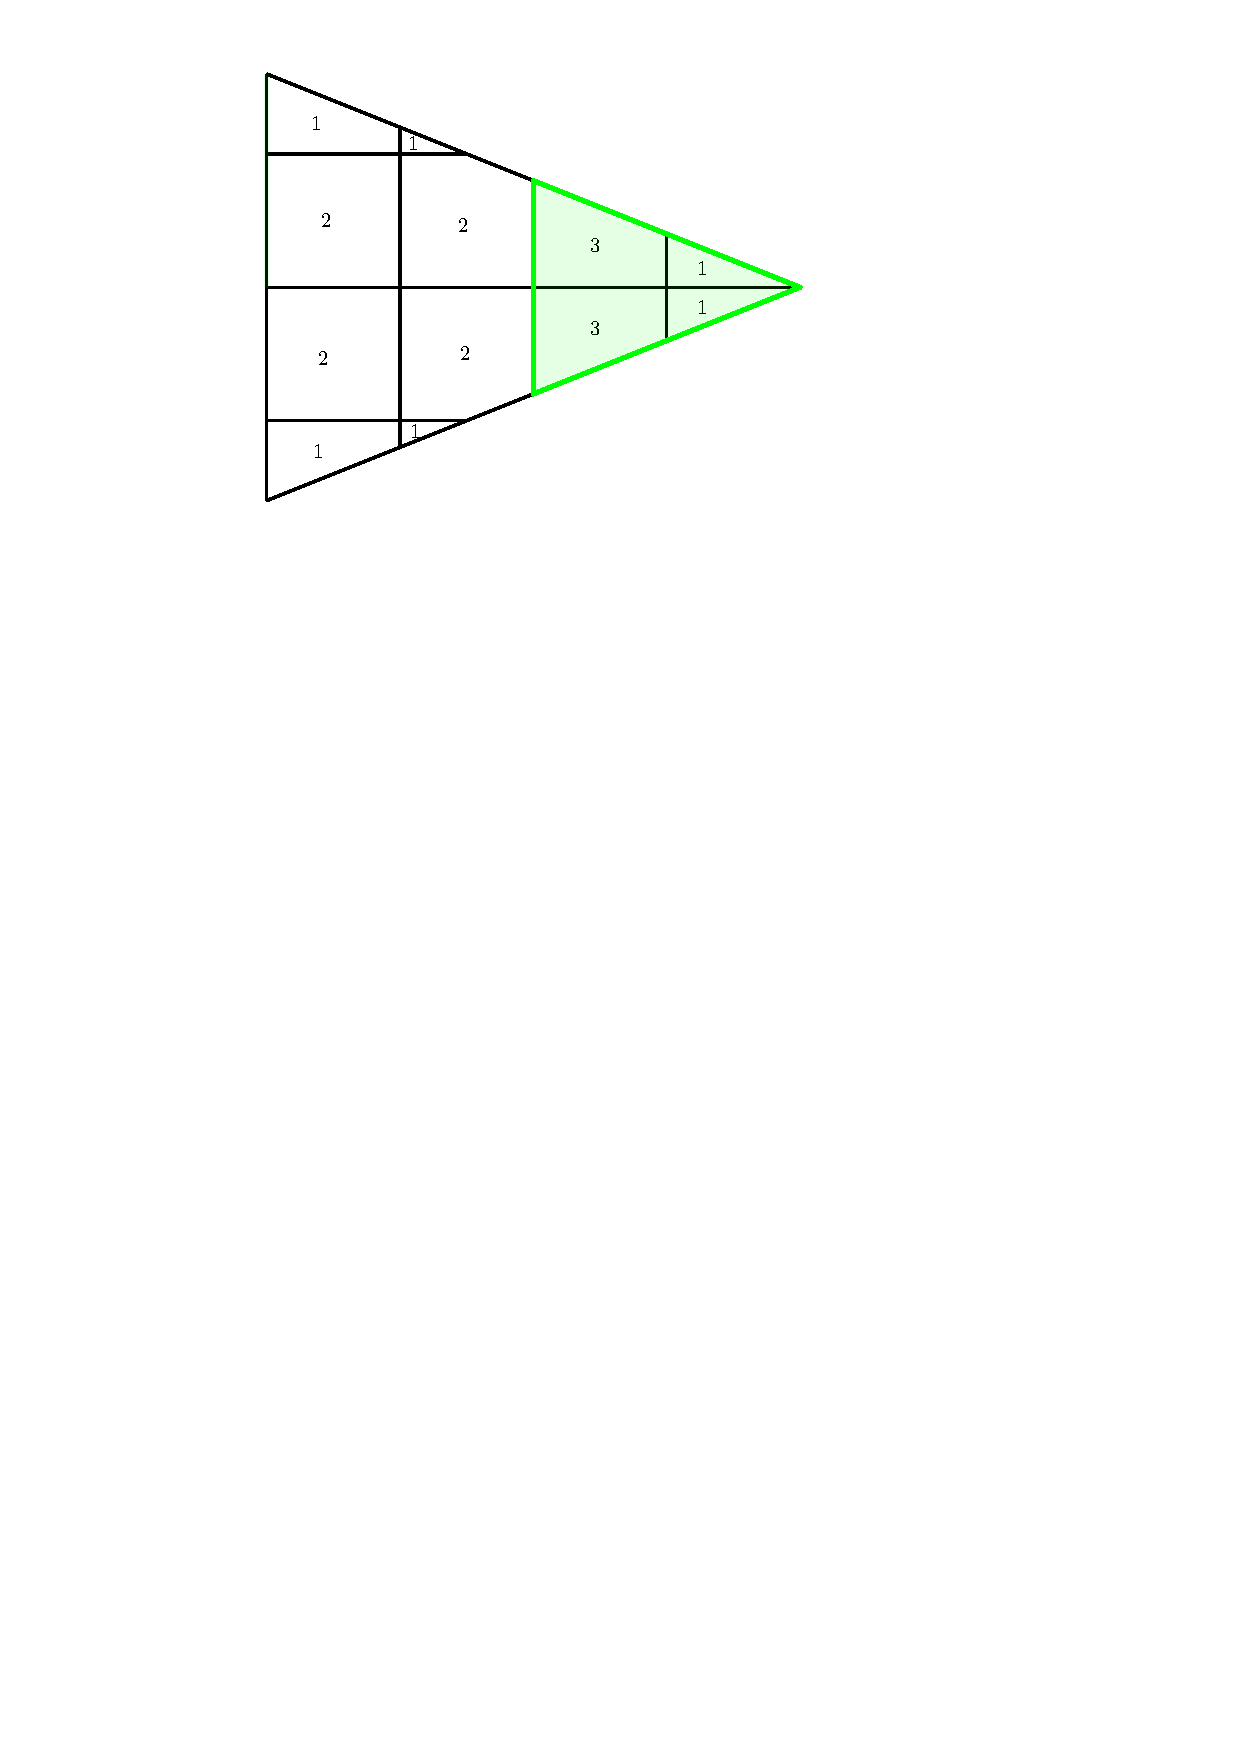
\includegraphics[width=.24\textwidth]{figs/numoverlaps5.pdf} \label{fig:numoverlaps4}}
%	\hfill
%	\subfloat[]{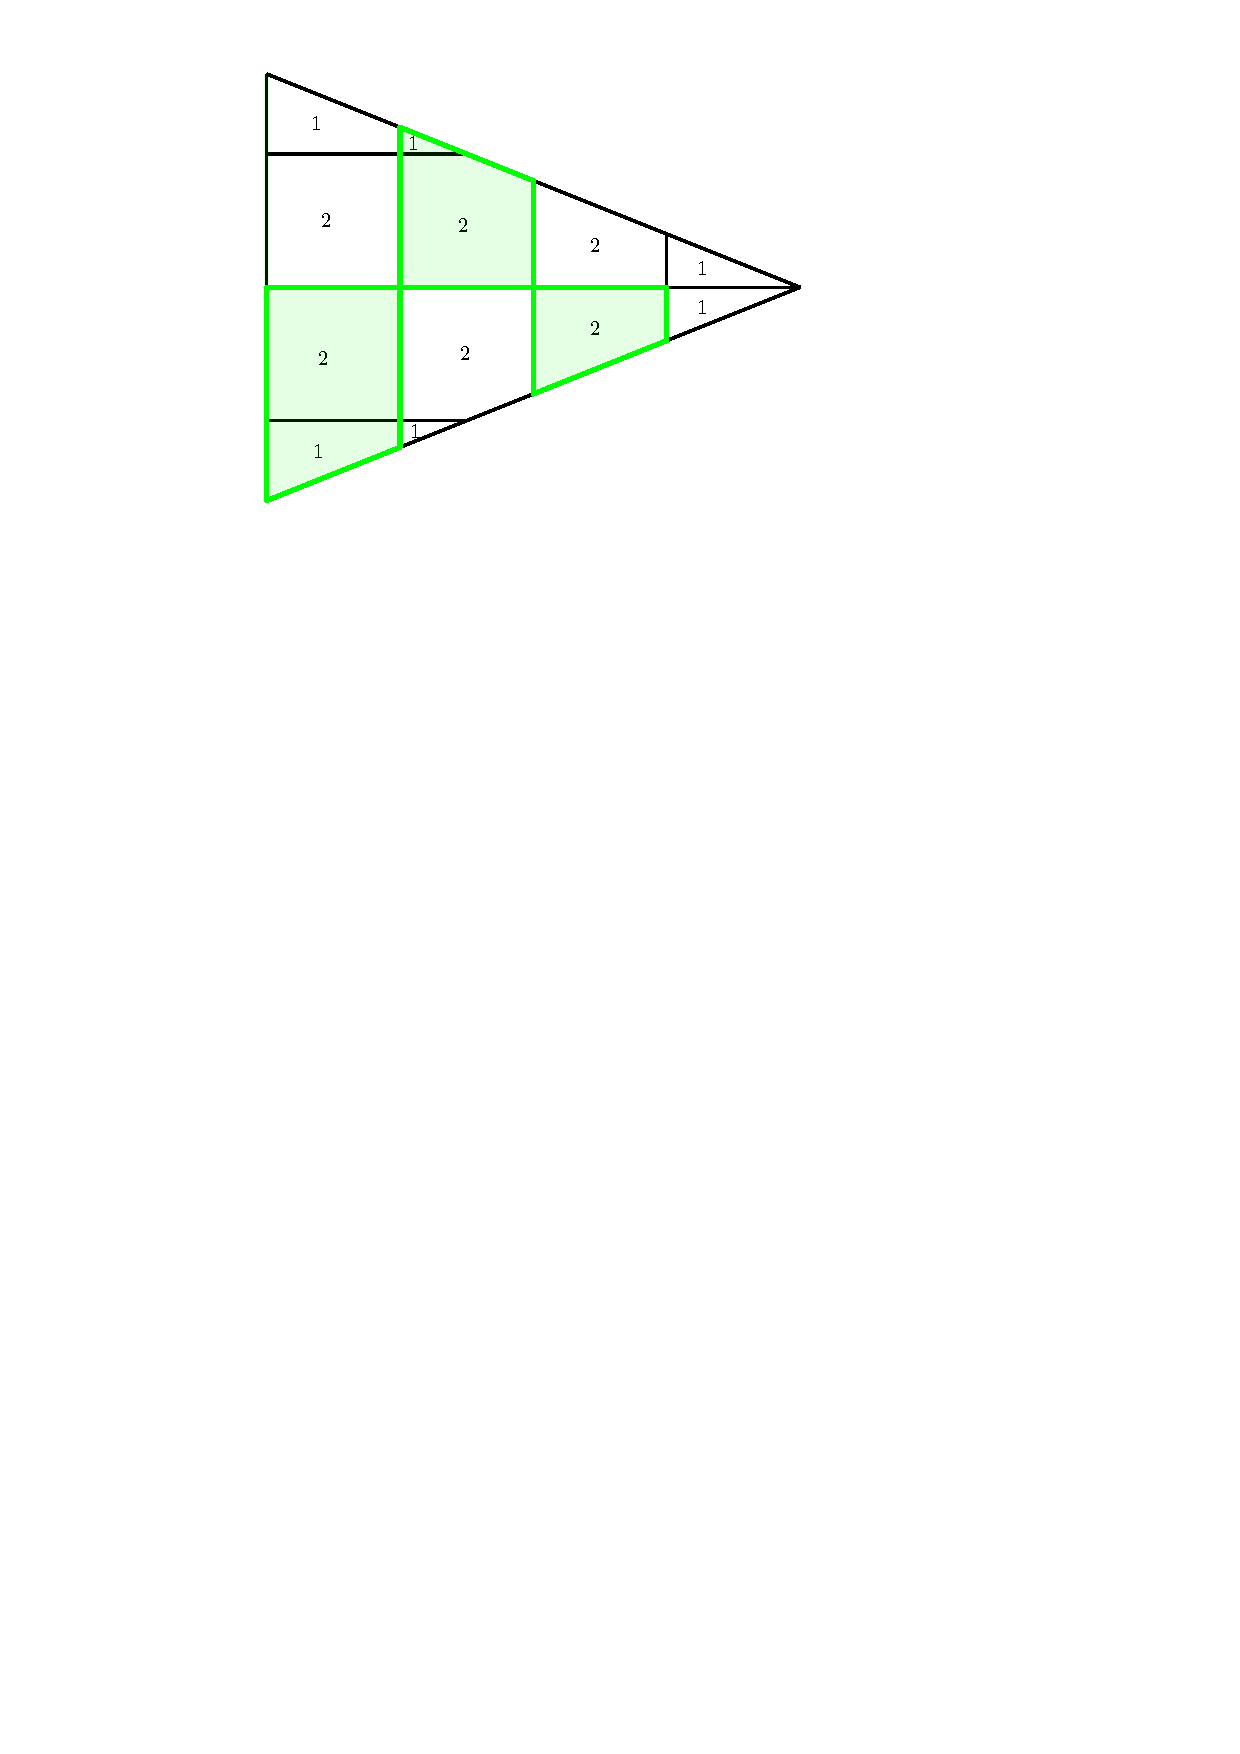
\includegraphics[width=.24\textwidth]{figs/numoverlaps2.pdf} \label{fig:numoverlaps2}}
%    \hfill
%	\subfloat[]{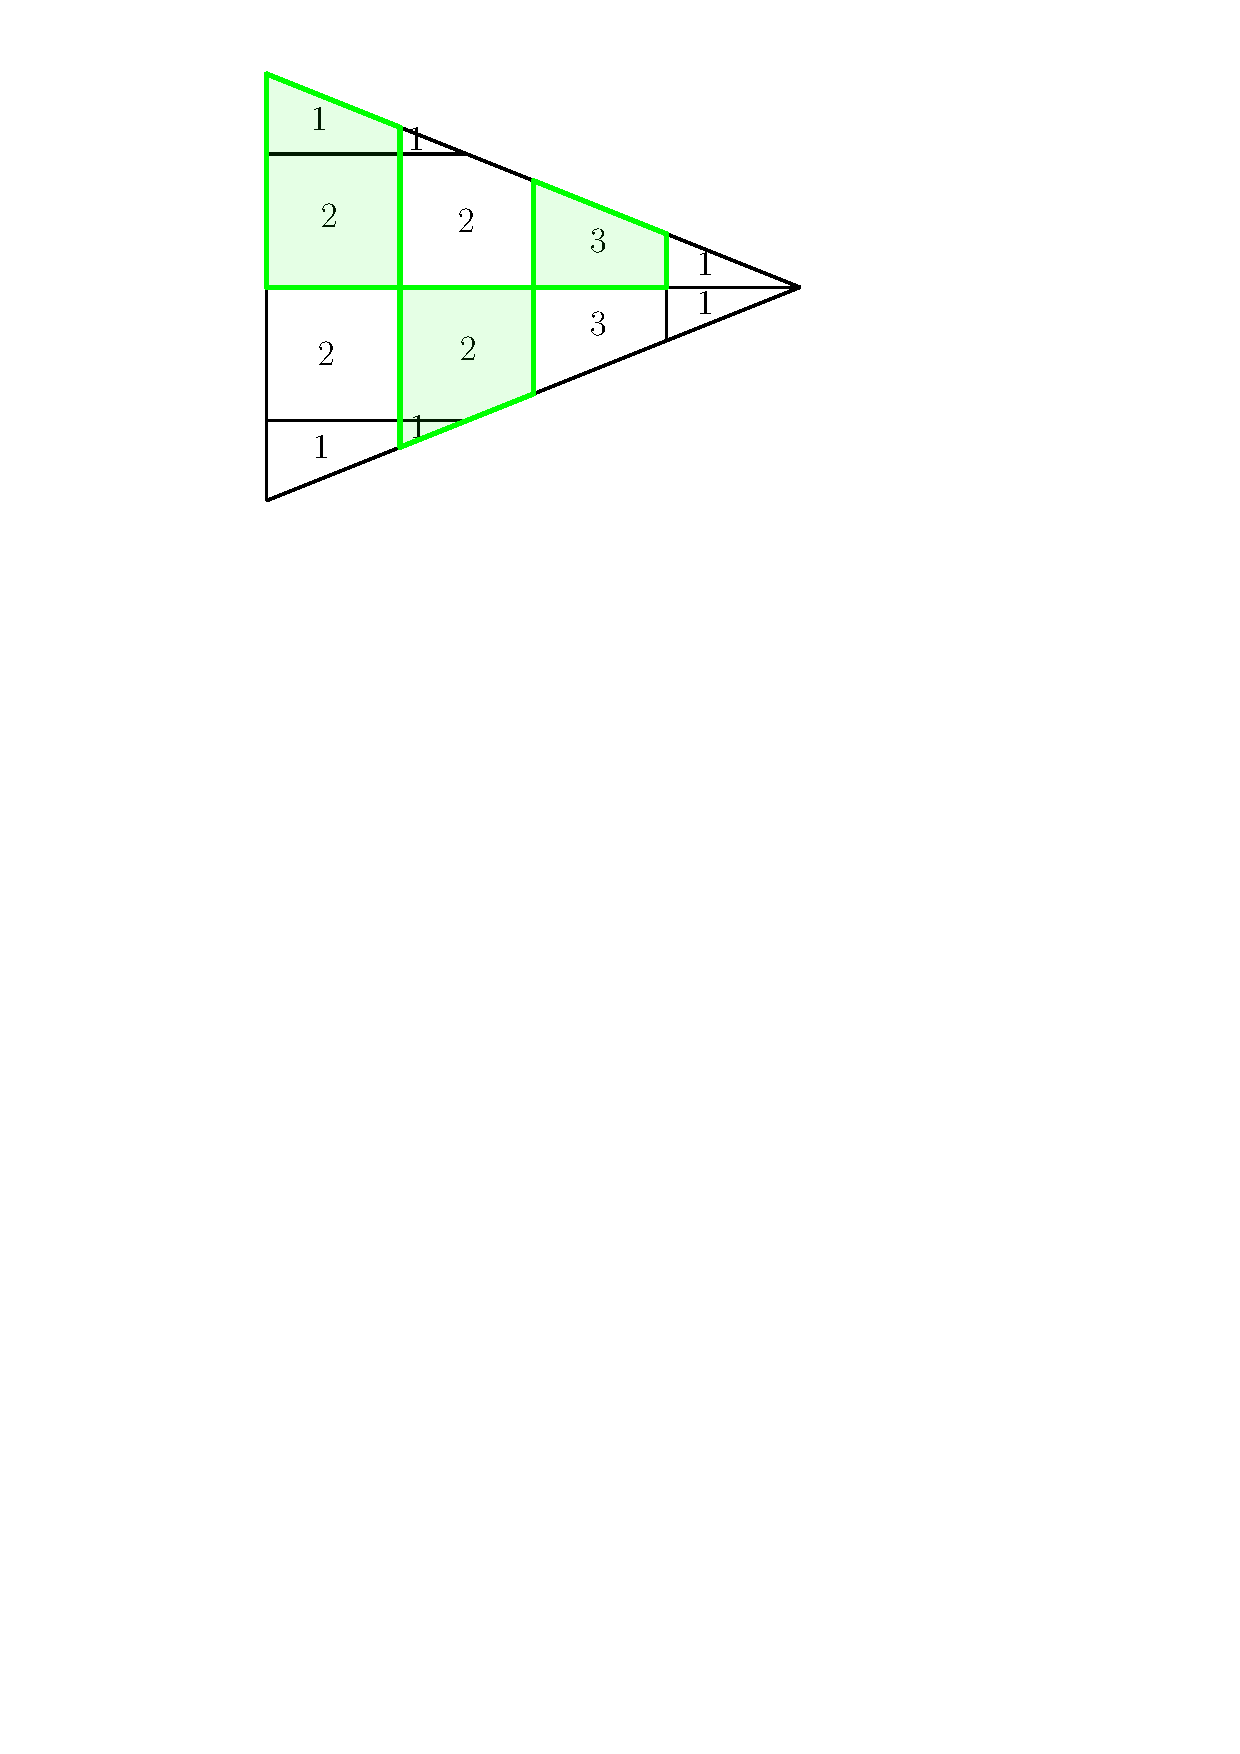
\includegraphics[width=.24\textwidth]{figs/numoverlaps3.pdf} \label{fig:numoverlaps3}}
%	\caption{\sf All merging neighborhoods on an example cut cell mesh (in green).  We display the number of overlapping merging neighborhoods on each cell. Note, in figure \ref{fig:numoverlaps4}, there are two merging neighborhoods that occupy the same location, one per small cell in the right corner.} \label{fig:overlappingneighs}
%\end{figure}
But a full cell can be part of 
two (or more)  merging neighborhoods  if it is placed next to 
one (or more)  tiny cut cells. This is the case for the left cell in figure
\ref{fig:neighborhoods}. The full cell is its own merging neighborhood, 
as well as being part of the cut cell's neighborhood. Thus the full cell has a
count of 2, and the cut cell has a count of 1.
%An example is shown in
%figure \ref{fig:2nborTile}. The cells in green are part of two
%neighborhoods, and those in red are part of three.   

Most full
cells are only members of their own tile and will have a count of one.
Only cells within a narrow band of the cut cells will have a count
larger than one.

\item
{\bf Each neighborhood computes its weighted centroid and volume.}

Each merging neighborhood computes the  volume and centroid weighted by
the number of neighborhoods it belongs to.  Note that this is generally
\textit{not} the volume or centroid of the cell $i,j$, unless the count is one, or
all counts in the neighboorhood are equal and therefore cancel.  
The neighborhood's weighted volume is defined as
\begin{equation}
\label{voldef}
{\widehat V}_{i,j} =  \sum_{k \in M_i } \,  \frac{V_k}{N_k},
\end{equation}
and the weighted centroid of the merging neighborhood is defined as
\begin{equation}
\label{centroiddef}
({\widehat x}_{i,j},{\widehat y}_{i,j}) = \frac{1}{\widehat V_{i,j}} \sum_{k \in M_i } \,  \frac{V_k}{N_k}(x_k,y_k),
\end{equation}
where $k$ is a multi-index ranging over the neighbors of cell $i,j$ included in its merging tile.  The difference between $(x_{i,j}, y_{i,j})$ and $(\widehat{x}_{i,j}, \widehat{y}_{i,j})$ is illustrated in figure \ref{fig:centroids}.


\begin{figure}[h]
    \centering
    \hspace*{.5in}
    \subfloat[]{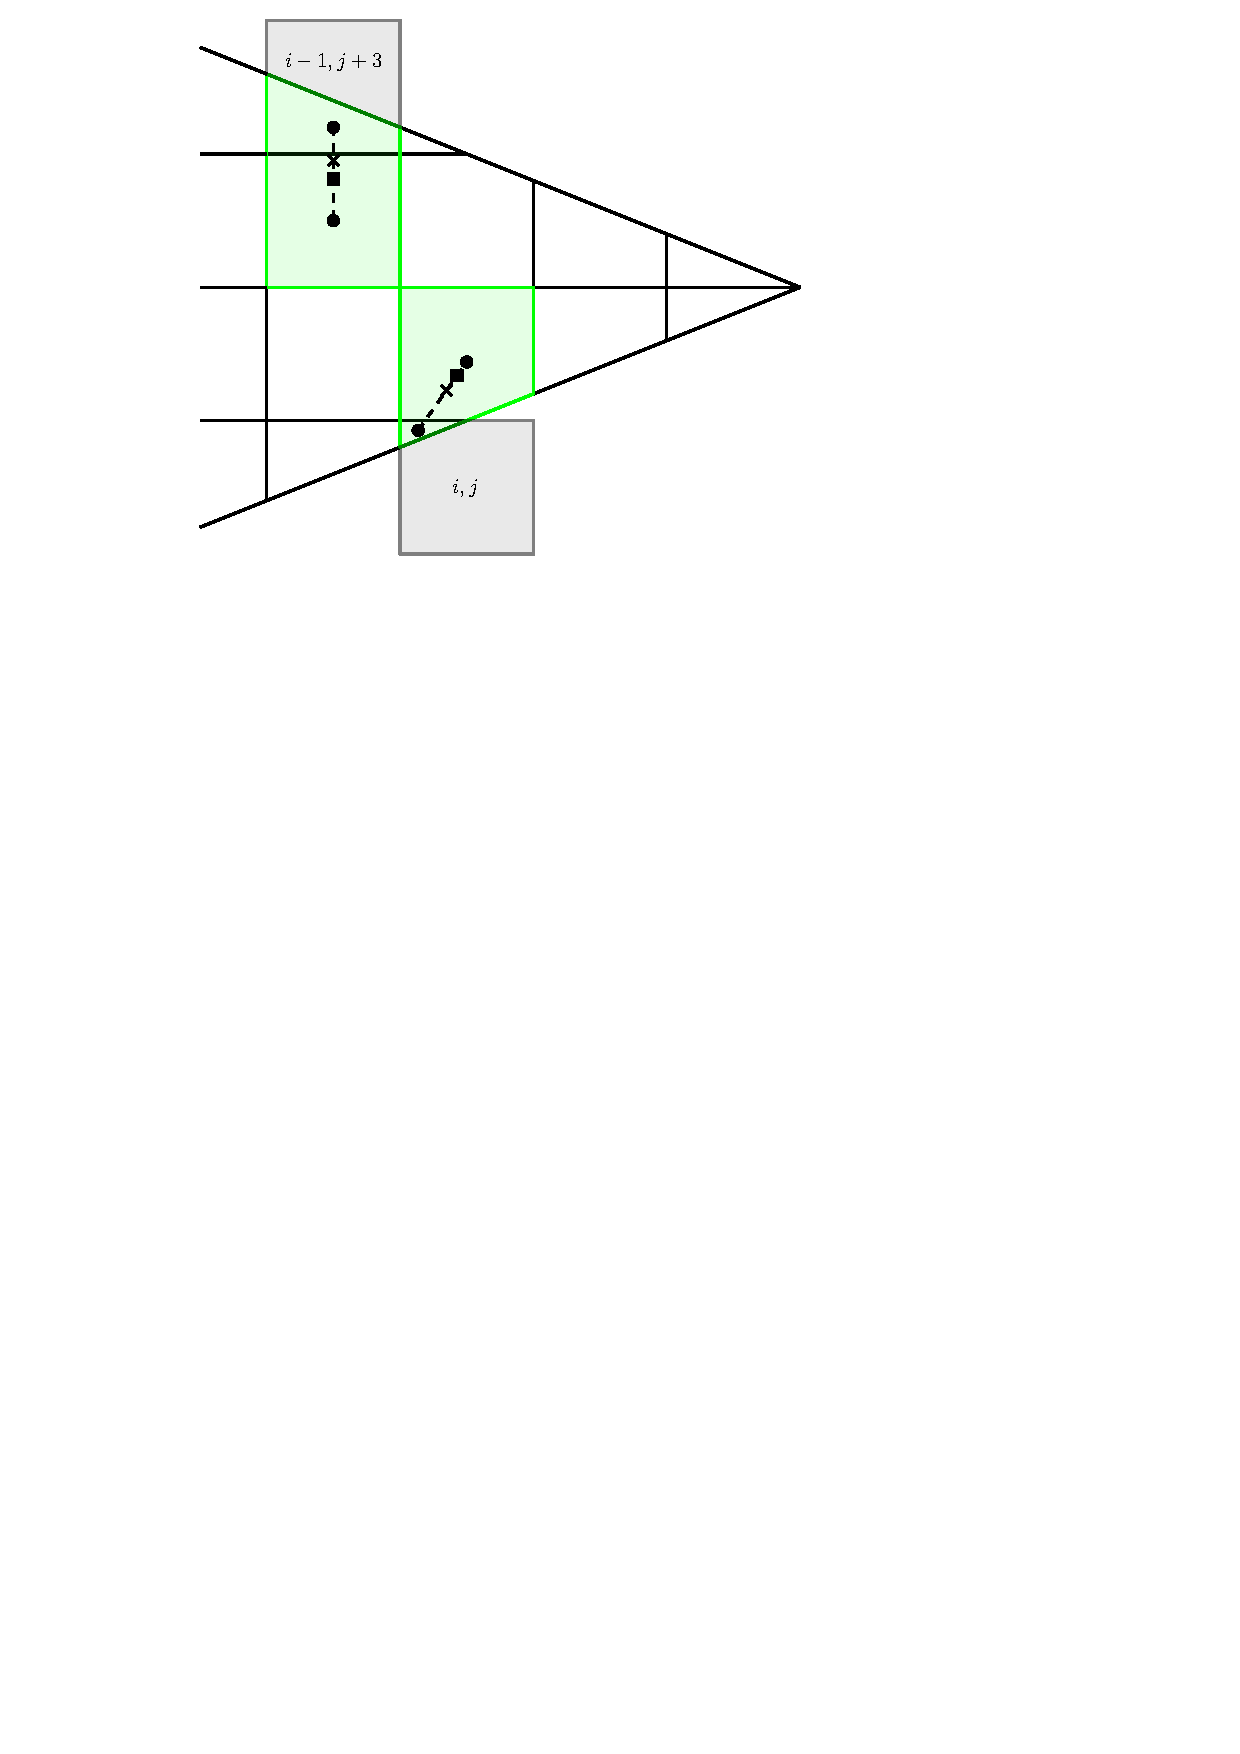
\includegraphics[width=0.35\linewidth]{figs/centroids3.pdf}} \hfill
    \subfloat[]{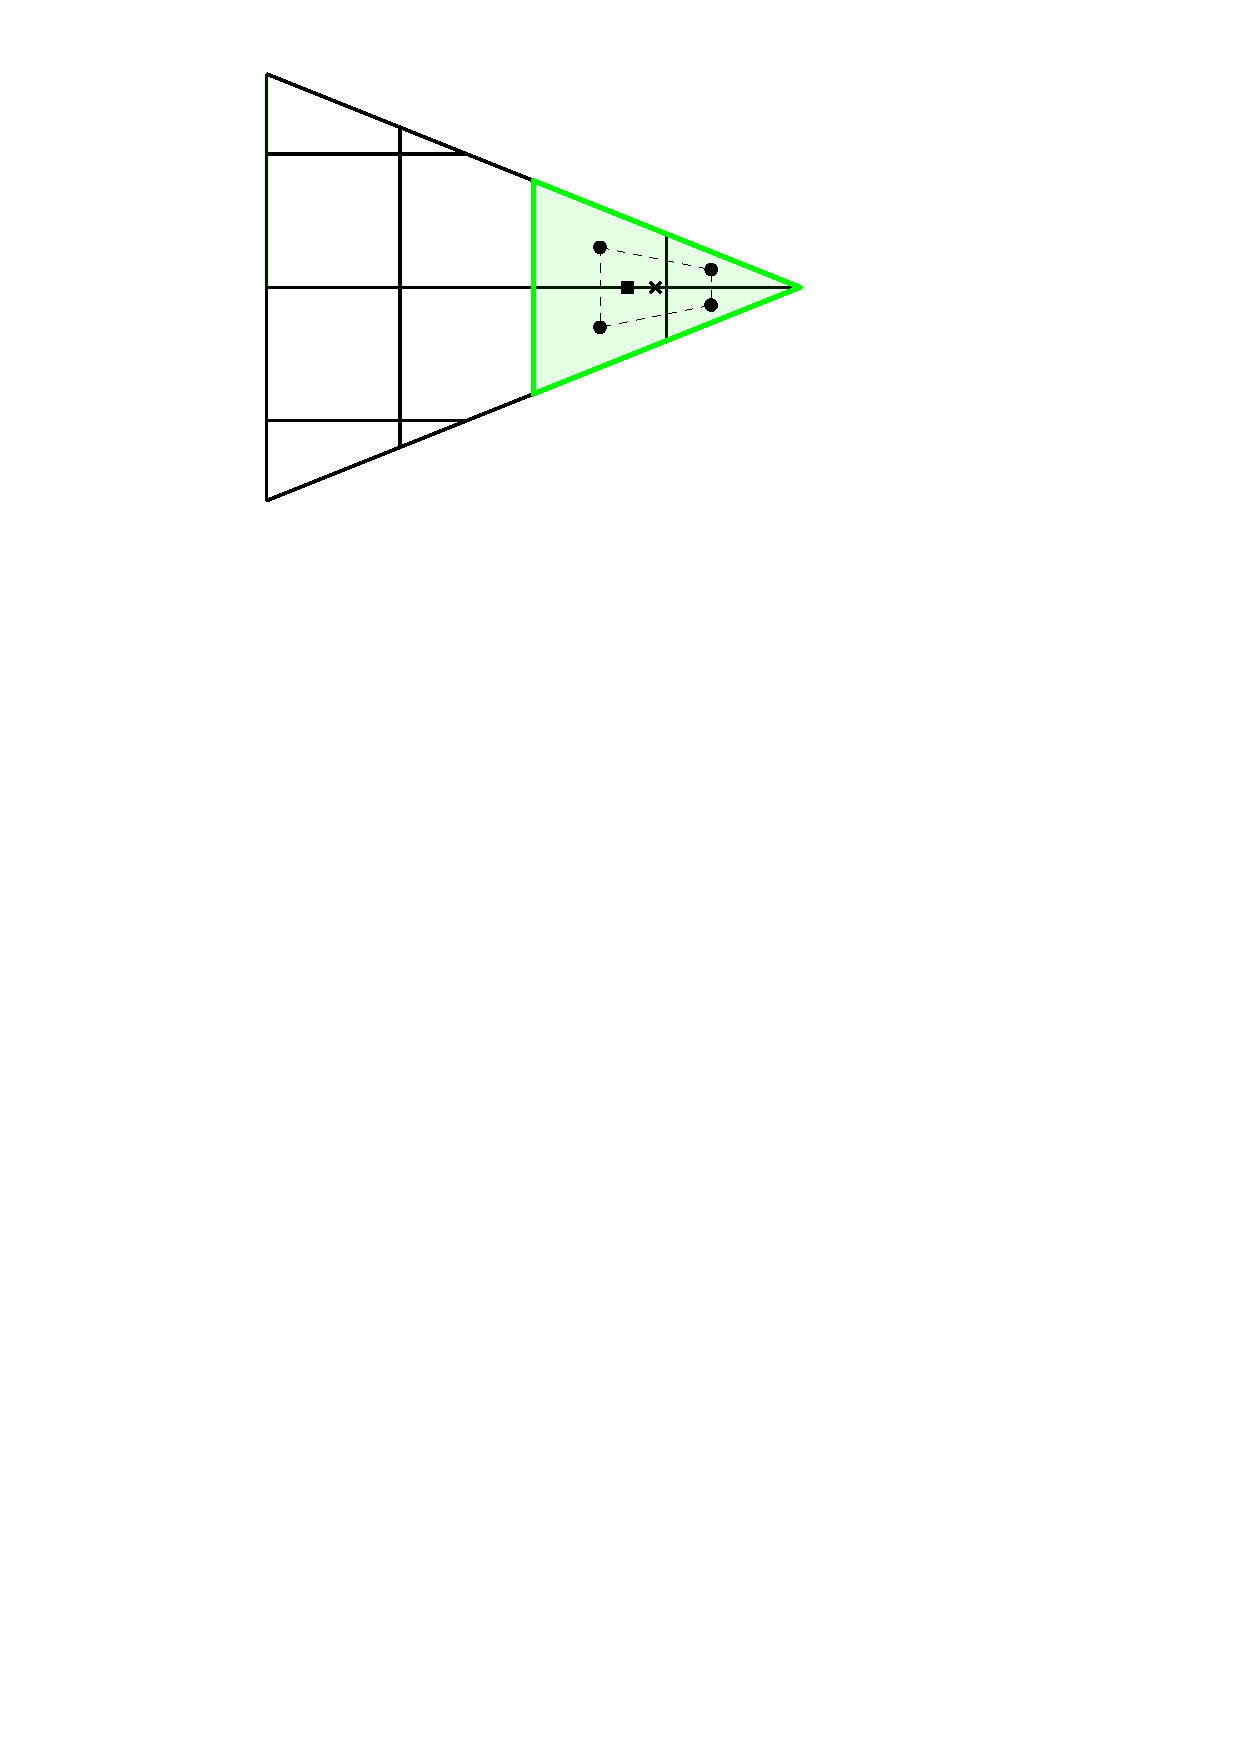
\includegraphics[width=0.35\linewidth]{figs/centroids4.pdf}}
    \caption{\sf The centroids of the Cartesian and cut cells are indicated with a solid circle ($\bullet$).  The centroids and weighted centroids of the merging neighborhoods are indicated with a square ($\blacksquare$) and a cross ($\times$), respectively. Note that the centroids and weighted centroid of the cut cell neighborhoods do not necessarily coincide.}
    \label{fig:centroids}
\end{figure}

\end{itemize}

% \begin{figure}[h!]
% \begin{center}
% 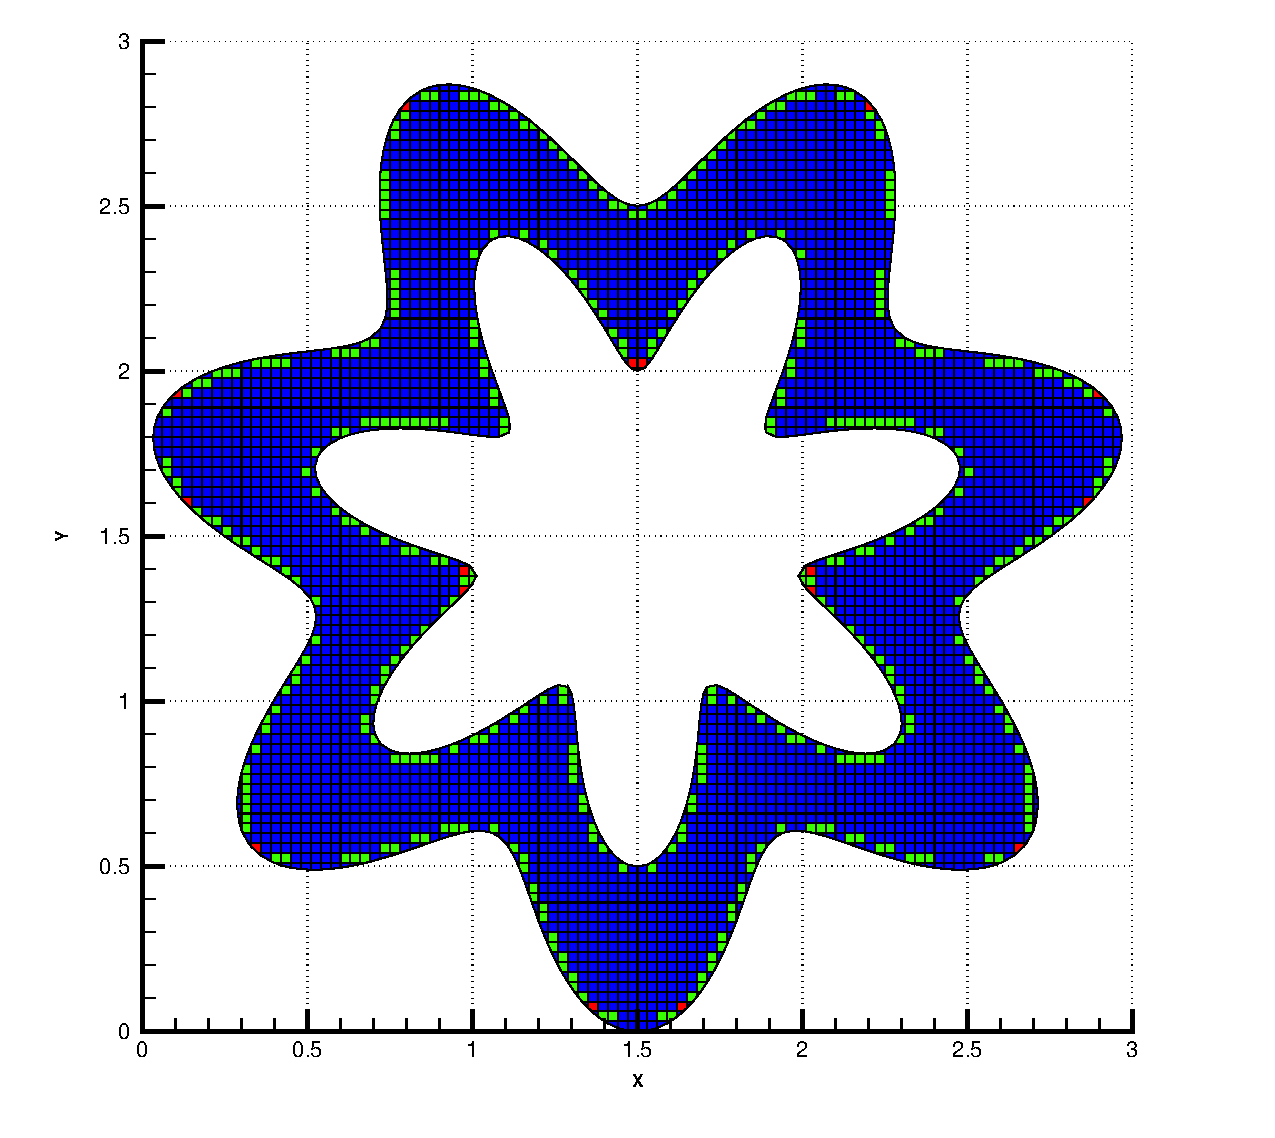
\includegraphics[width=4.5in]{figs/waveynumhoods.eps}
% \caption{\sf Domain from example XX.  Figure shows how many
% neighborhoods each cell belongs to: 
% one (white), two (blue), or three (red).
% The full example is shown in section \ref{sec:compResults}.}
% \label{fig:2nborTile}
% \end{center}
% \end{figure}

These three steps can be part of a preprocessing step since they do not
depend on the computed solution. However for moving geometry they would
be done at each step.

\vspace*{.1in}
\subsection{State Redistribution Postprocessing }
Using the merging tiles and the cell counts, the  state redistribution
algorithm is applied after one step or stage of the base scheme,
$$
\widehat{U} = U^n + \Delta t \, L(U^n),
$$
where $L$ is given by one of the finite volume schemes
described in section \ref{sec:basefv}. The variable $\widehat{U}$ refers to the
provisionally updated value before SRD postprocessing.

\begin{enumerate}
\item
{\bf Compute the volume-weighted,  count-weighted solution for all
merging tiles.}   

\vspace*{.1in}
The solution $\widehat{Q}$ for each neighborhood is computed,
\begin{equation}
\label{tiledef}
\widehat{Q}_{i,j} =  \frac{1}{{\widehat V}_{i,j}} \, \sum_{k \in M_i} \,  
\frac{V_k}{N_k}  \,\,  \widehat{U}_k
\end{equation}
where the volume ${\widehat V}_{i,j}$ is the 
similarly weighted merging tile volume of eq. \eqref{voldef}.
Recall that $M_{i,j}$ is the set of cell indices in the cell $(i,j)$ merging
neighborhood, and  
$k$ is  a multi-index ranging over the neighbors 
of cell $(i,j)$ included in its merging tile.

In words, the contribution of each cell is divided by the number of neighborhoods 
it is part of (i.e. its count). 
Most full cells will have ${\widehat V}_{i,j} = V_{i,j}$, 
and $\widehat{Q}_{i,j}  = \widehat{U}_{i,j}$, since they have a count of one.
At the other extreme, if all cells merged with the same number of neighbors, the $N_k$'s
would cancel, and the resulting solution would be the standard volume-weighted
solution over the included cells. 

\item
{\bf Compute and limit a gradient for each merging tile.}

\vspace*{.1in}
A gradient needs to be computed for each cut cell neighborhood. This will be needed
to accurately update the provisional solution in the next step.
A least squares procedure  similar to the one used in eq.~\eqref{eqn:lls} 
for the finite volume update of the cut cells is an 
obvious choice.  

We use a 3-by-3 neighborhood around $(i,j)$, ignore solid cells, and fit a least
squares solution using the weighted centroids.
As in eq. \eqref{eqn:lls}, the reconstruction on the merged 
neighboorhood is of the form
\begin{equation}
\widehat{q}(x,y) = \widehat{Q}_{i, j} + \widehat{\sigma}_{x,i,j}(x - \widehat{x}_{i,j}) + \widehat{\sigma}_{y,i,j}(y - \widehat{y}_{i,j}),
\end{equation}
where $\widehat{Q}_{i, j}$ is the solution average from eq. \eqref{tiledef} and $(\widehat{\sigma}_{x,i,j},\widehat{\sigma}_{y,i,j})$ is 
the gradient on the merging neighborhood.
The quantities $(\widehat{\sigma}_{x,i,j},\widehat{\sigma}_{y,i,j})$ satisfy in the least squares sense
\begin{equation}\label{eqn:linrecon}
\widehat{\sigma}_{x,i,j}(\widehat{x}_{k} - \widehat{x}_{i,j}) + \widehat{\sigma}_{y,i,j}(\widehat{y}_{k} - \widehat{y}_{i,j})= \widehat{Q}_{k} - \widehat{Q}_{i, j} \quad \forall k \in R_{i,j},
\end{equation}
Note that eq. \eqref{eqn:linrecon} uses the merging tile's weighted centroid
$(\widehat{x}_{i,j},\widehat{y}_{i,j})$ instead of the cell centroid. 
We use 
$W_{i,j}$ to refer to the set of indices of neighborhoods used for reconstruction,
since it need not be the same as the $R_{i,j}$ used in the cut cell gradient
reconstruction. DO I HAVE NOTATION RIGHT


%The gradient on the merging neighborhood $(\widehat{\sigma}_{x,i,j},\widehat{\sigma}_{y,i,j})$ satisfies in the least squares sense
%\begin{equation}\label{eqn:linrecon}
%\widehat{\sigma}_{x,i,j}(\widehat{x}_{k} - \widehat{x}_{i,j}) + \widehat{\sigma}_{y,i,j}(\widehat{y}_{k} - \widehat{y}_{i,j})= \widehat{Q}_{k} - \widehat{Q}_{i, j} \quad \forall k \in R_{i,j},
%\end{equation}
%where $R_{i,j}$ is the set of indices of neighborhoods used for reconstruction 
%on merging neighborhood $i$.  That is, the reconstruction on the merged neighborhood is the linear function of best fit through the points $(\widehat x_k, \widehat y_k, \widehat Q_k)$ $\forall k \in R_{i,j}$ and that passes exactly through $(\widehat x_{i,j}, \widehat y_{i,j}, \widehat{Q}_{i,j})$.


We use a 3-by-3 neighborhood around the tile for cell $(i,j)$, again
ignoring solid cells.
However it could happen that the 3-by-3 neighborhood does not have enough cells,
or that the centroids are too close to each other to compute a 
well-conditioned gradient.
This is the case in figure \ref{fig:tooclose}, which shows the location of the
centroids in $y$ are too close, but they are well-separated 
in the  $x$ direction. 
If the weighted centroids are not at least $0.5\,\Delta x$  and $0.5\,\Delta y$ 
apart in the $x$ or $y$ direction then we increase the stencil size for the 
gradient computation.  For example, if the weighted centroids are too close in the $x$ 
direction, but not the $y$ direction, then the $5\times 3$ tile is used as the 
reconstruction neighborhood.  Similarly, if the weighted centroids are too 
close in the $y$ direction, but not the $x$ direction, then the $3\times 5$ tile is 
used as the reconstruction neighborhood.  The neighborhood size is increased until the 
distance constraint is satisfied in both directions.  In figure \ref{fig:tooclose},
the appropriate reconstruction neighborhood is $3\times 5$ reconstruction tile.

\begin{figure}
    \centering
    \subfloat[]{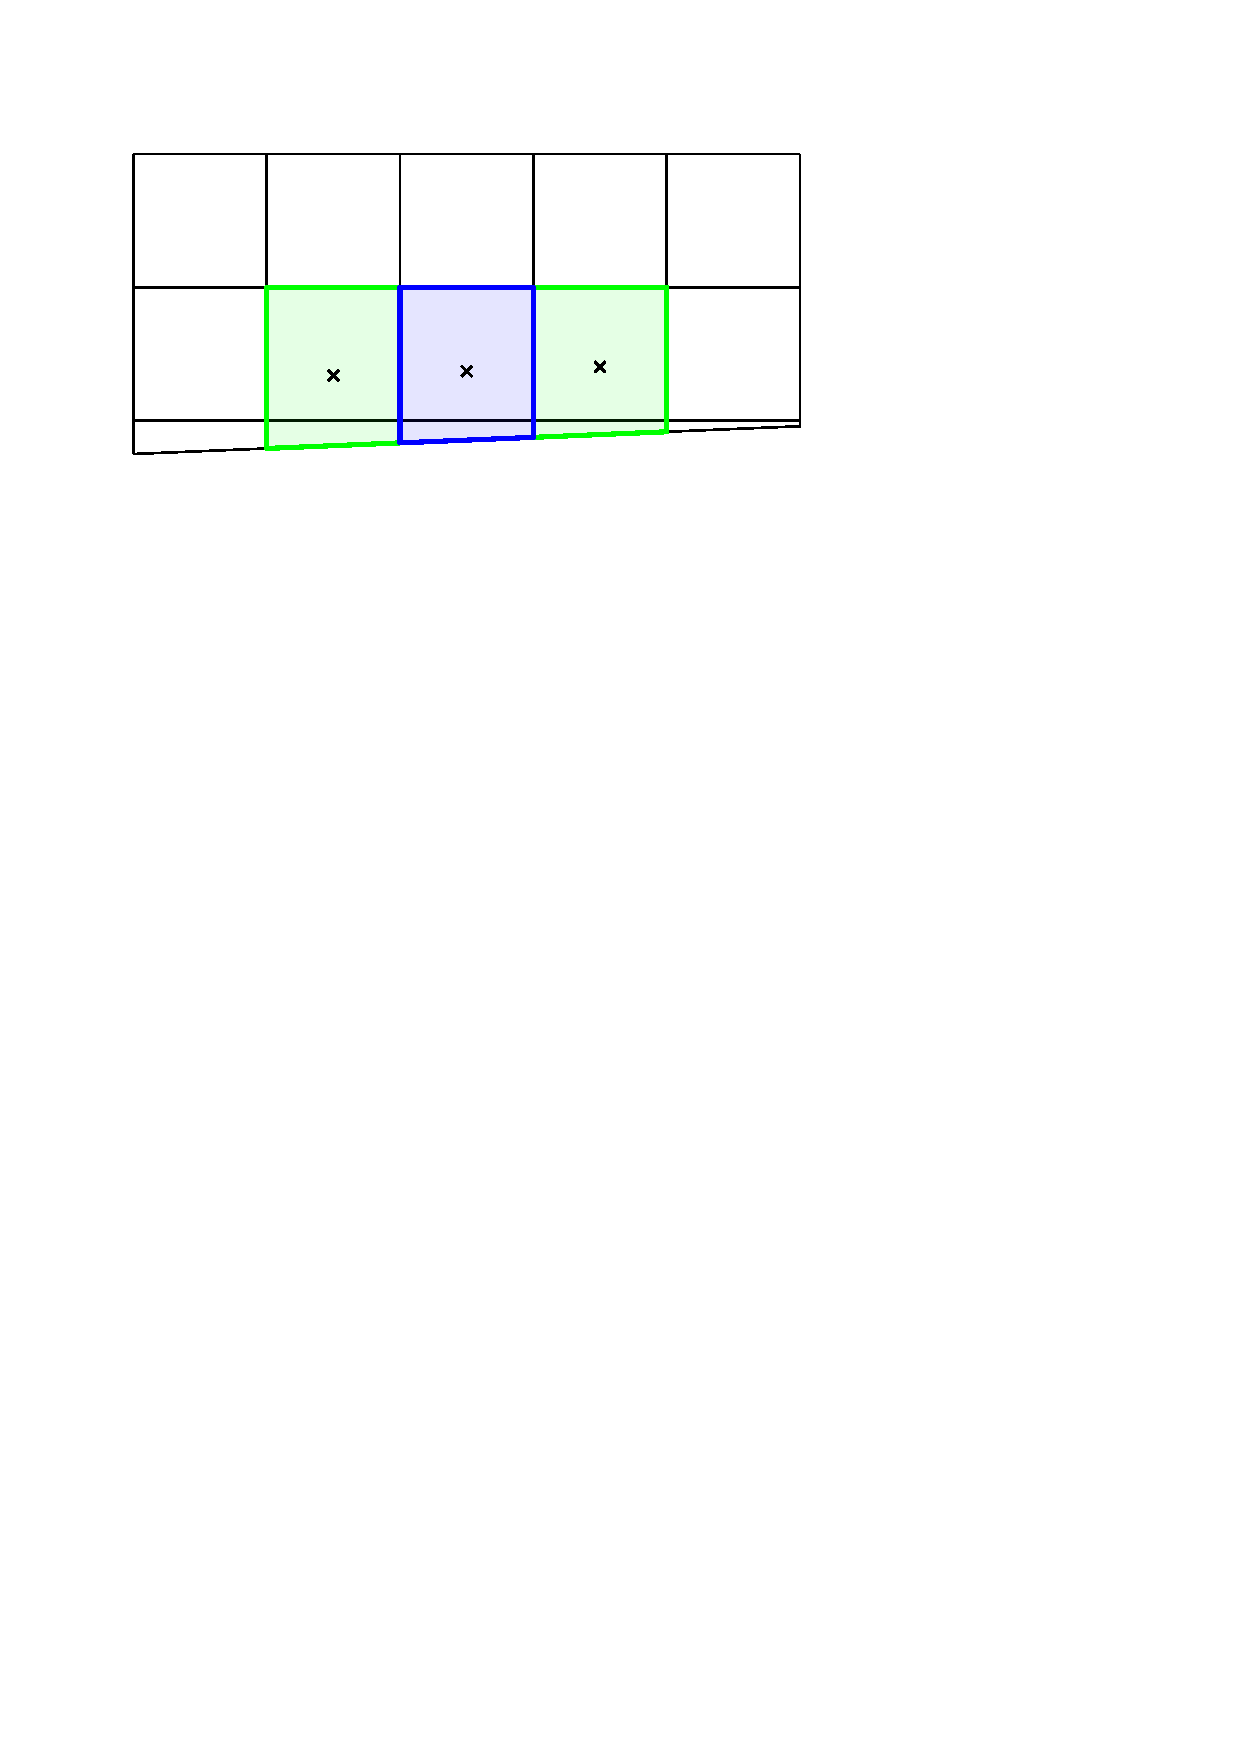
\includegraphics[width=0.40\linewidth]{figs/tooclose2.pdf}} \hfill
    \subfloat[]{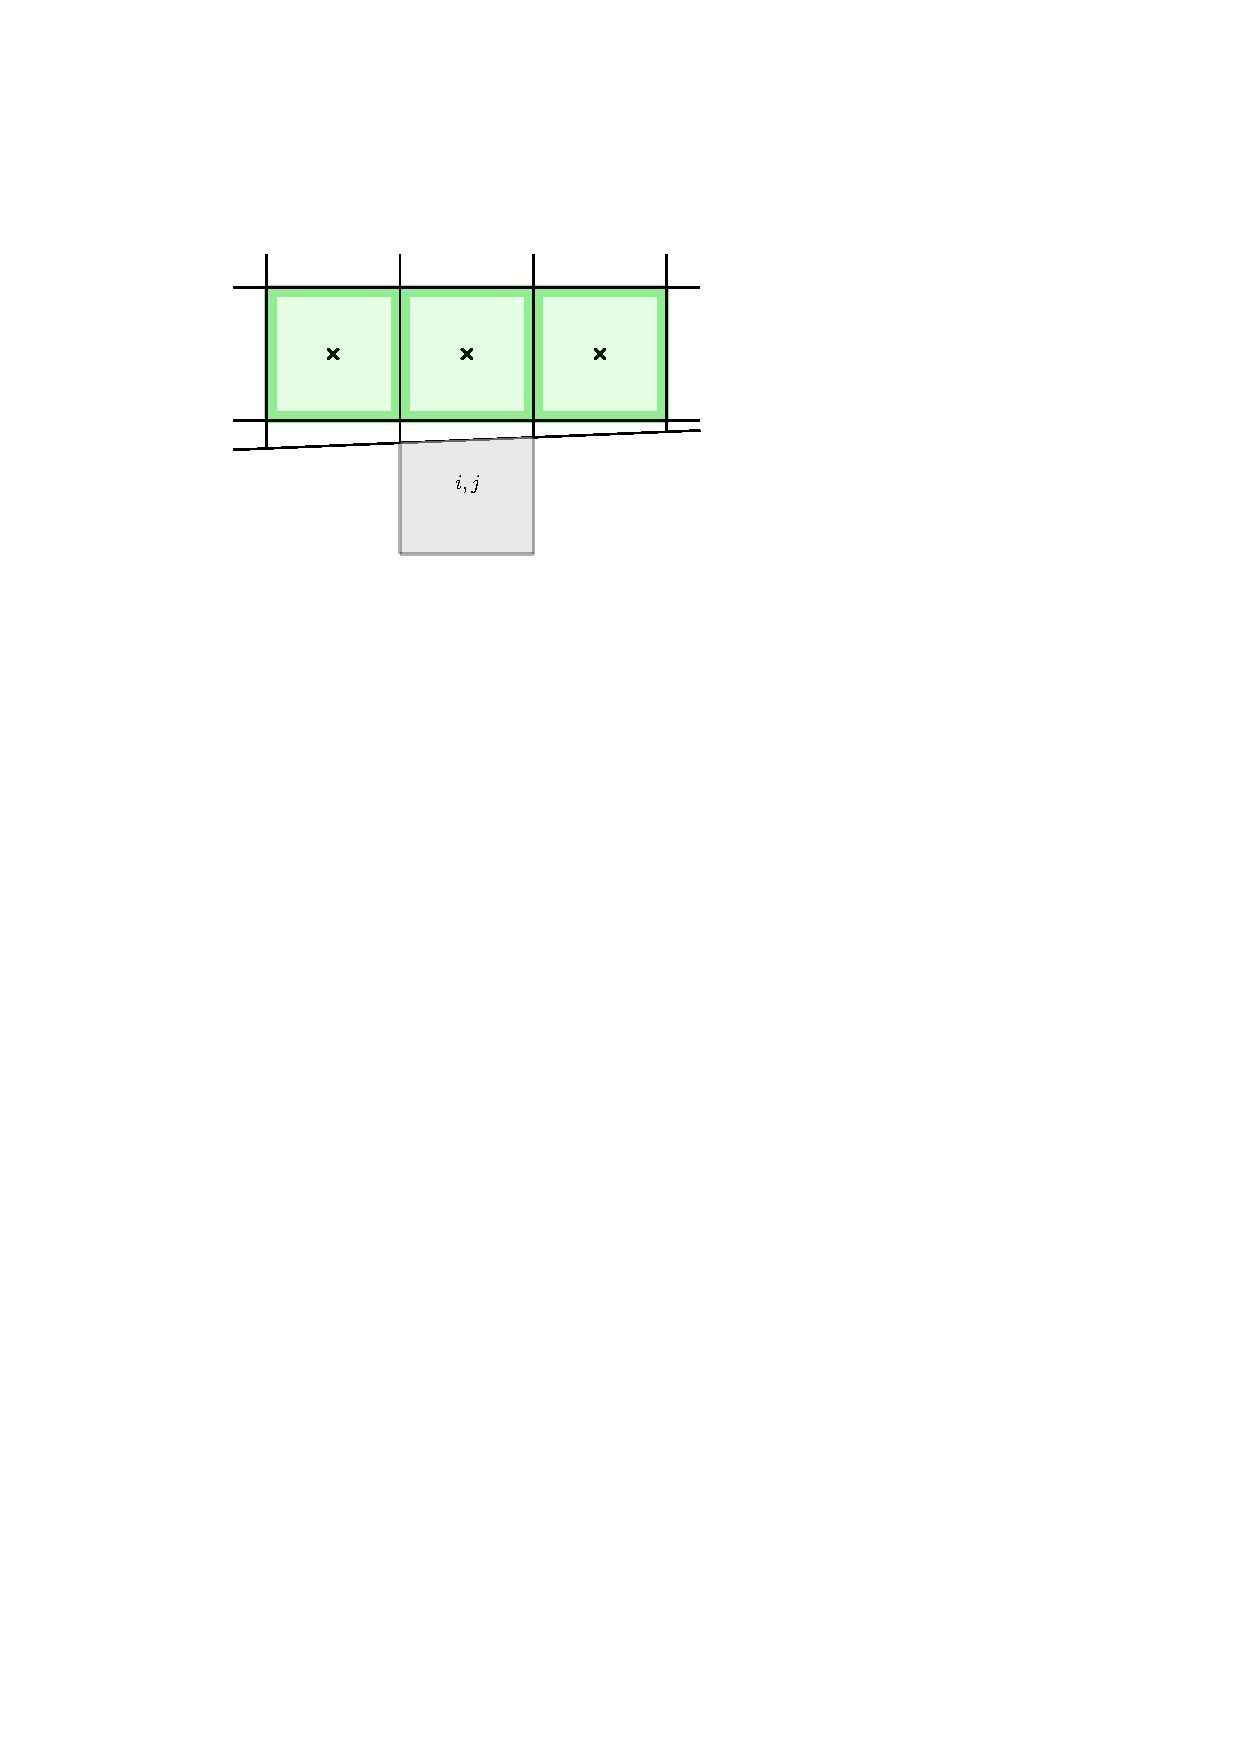
\includegraphics[width=0.40\linewidth]{figs/tooclose1.pdf}} 
    \caption{\sf On the left, the blue cell's $3\times3$ gradient reconstruction 
    stencil  is highlighted in green. On the right, cell $(i,j+1)$ has a
    stencil highlighted in green, for computing the gradient in $x$. 
    The weighted centroids are indicated with a cross ($\times$).
    They are TOO CLOSE NEED LARGER NEIGHBORHOOD (WHAT DOES THIS SHOW)}
    \label{fig:tooclose}
\end{figure}

Note that full cells, where the merged  solutions $\widehat{Q} =
\widehat{U}$ (the
provisionally updated solution), do not need a gradient. The solution will only be
evaluated at the cell centroid, which is the same as the neighborhood centroid, so
no offsets will be computed. However the merging neighborhood of the cut cell will
also contributed to the full cell.

To limit the gradient we again apply BJ, this time over the neighboring merging tiles 
instead of neighboring cells as in eq. \eqref{eqn:bj}.  NEED TO TRY USING LP TOO


\item
{\bf The merging neighborhoods replace the provisionally computed solution 
with the merged tile solution on the cut cells and adjacent full cells.} 

\vspace*{.1in}
The final solution on cell $(i,j)$ is given by the average of the 
reconstructed polynomials that overlap the cell. Letting $W_{i,j}$ be the list of
indices of these overlapping tiles. Then the update for cell $(i,j)$ is
\begin{equation} \label{eqn:final_update_linear}
U^{n+1}_{i,j} := \frac{1}{N_{i,j}}\sum_{k \in W_{i,j}}\hat{q}_{k}(x_{i,j},y_{i,j}).
\end{equation}
The solution on merging neighborhood $k \in W_{i,j}$ is evaluated at $(i,j)$'s 
physical centroid, $(x_{i,j},y_{i,j})$, given by $\hat{q}_{k}(x_{i,j},y_{i,j})$.  

To use the example of figure \ref{fig:2nborTile}, the cut cell value
\begin{equation}
   U_{i,j}^{n+1} := \widehat{Q}_{i,j} 
   + ( x_{i,j} - \widehat x_{i,j}) \, \widehat{\sigma}_{x,i,j}
   + ( y_{i,j} - \widehat y_{i,j}) \, \widehat{\sigma}_{y,i,j}
\end{equation}
since cell $(i,j)$ only belongs to one neighborhood. The adjacent full cell
$(i,j+1)$ on the other hand belongs to two neighborhoods -- the one it 
shares with
the cut cell $(i,j)$ , and its own merging neighborhood.
So its solution at time $t^{n+1}$  becomes
\begin{equation}
\label{eqn:numhood2ex}
\begin{split}
   U_{i,j+1}^{n+1} \,=\, & \frac{1}{2} \, \widehat{q}_{i,j}(x_{i,j+1},y_{i,j+1})+ 
   \frac{1}{2} \,  \widehat{q}_{i,j+1}(x_{i,j+1},y_{i,j+1}), \\
   = &\frac{1}{2} \left
   (\widehat{Q}_{i,j} 
   + ( x_{i,j+1} - \widehat x_{i,j}) \, \widehat{\sigma}_{x,i,j}
   + ( y_{i,j+1} - \widehat y_{i,j}) \, \widehat{\sigma}_{y,i,j} \right ) + 
   \frac{1}{2} \, \widehat{Q}_{i,j+1} .
\end{split}
\end{equation}
The last term  in eq. \eqref{eqn:numhood2ex} has no gradient terms because the
centroids of the original cell and merged cell are identical.
The fraction $\frac{1}{2}$ is because cell $(i,j+1)$ is part of  two
neighborhoods, so each contributes half of the solution.
\end{enumerate}

One might at first think that only the cut cell needs to have its solution replaced
by the more stable update.  This would not be conservative however; the adjacent cell
also needs to be part of the update. In addition, each of these cells might also be part of
another neighborhood if the geometry curves, for example. So in the general case,
each contribution from a merging tile has to be weighted by the number of
neigborhoods it contributes to. 


The final update formula \eqref{eqn:final_update_linear} can easily be implemented with a 
nested for loop in algorithm \ref{alg:finalupdate}.  
The outer loop iterates over the merging neighborhoods $i,j$ and the inner loop 
iterates over each cell $k$ in merging neighborhood $i,j$.  Each merging 
neighborhood $(i,j)$ gives a contribution $ \hat{q}_{i,j}(x_{k}, y_k)/N_{k} $ to the 
cells $k$ that belong to it.

\begin{algorithm}[H]
\SetAlgoLined
$U^{n+1}(:,:) := 0$\\
 \ForAll{$i,j$}{
     \ForAll{$k \in M_{i,j}$}{
        $U^{n+1}_k := U^{n+1}_k + \hat{q}_{i,j}(x_{k}, y_k)/N_{k} $
     }
 }
 \caption{\sf Final solution update} \label{alg:finalupdate}
\end{algorithm}

\begin{figure}
	\subfloat[]{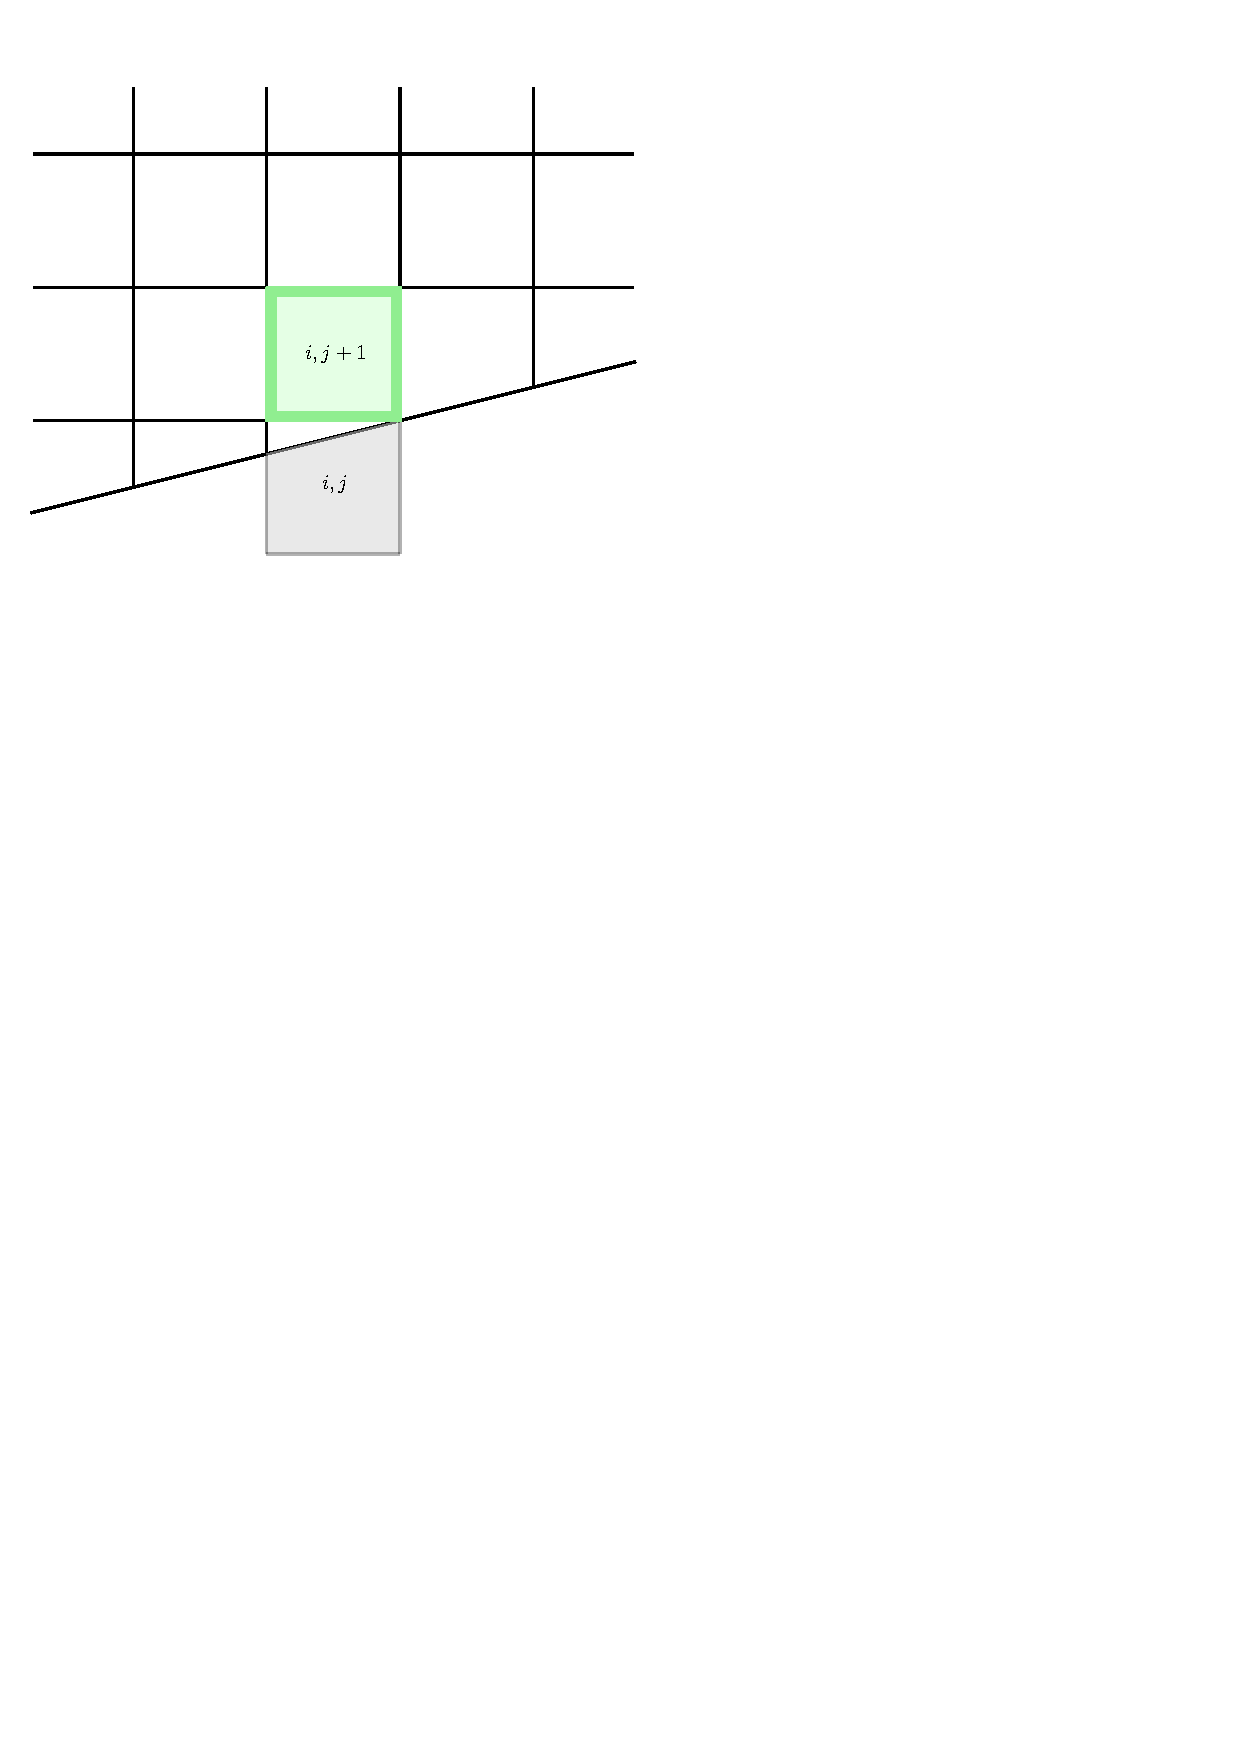
\includegraphics[width=0.40\textwidth]{figs/modelexample2D_1.pdf} \label{fig:2nborTile1}}
	\hfill
	\subfloat[]{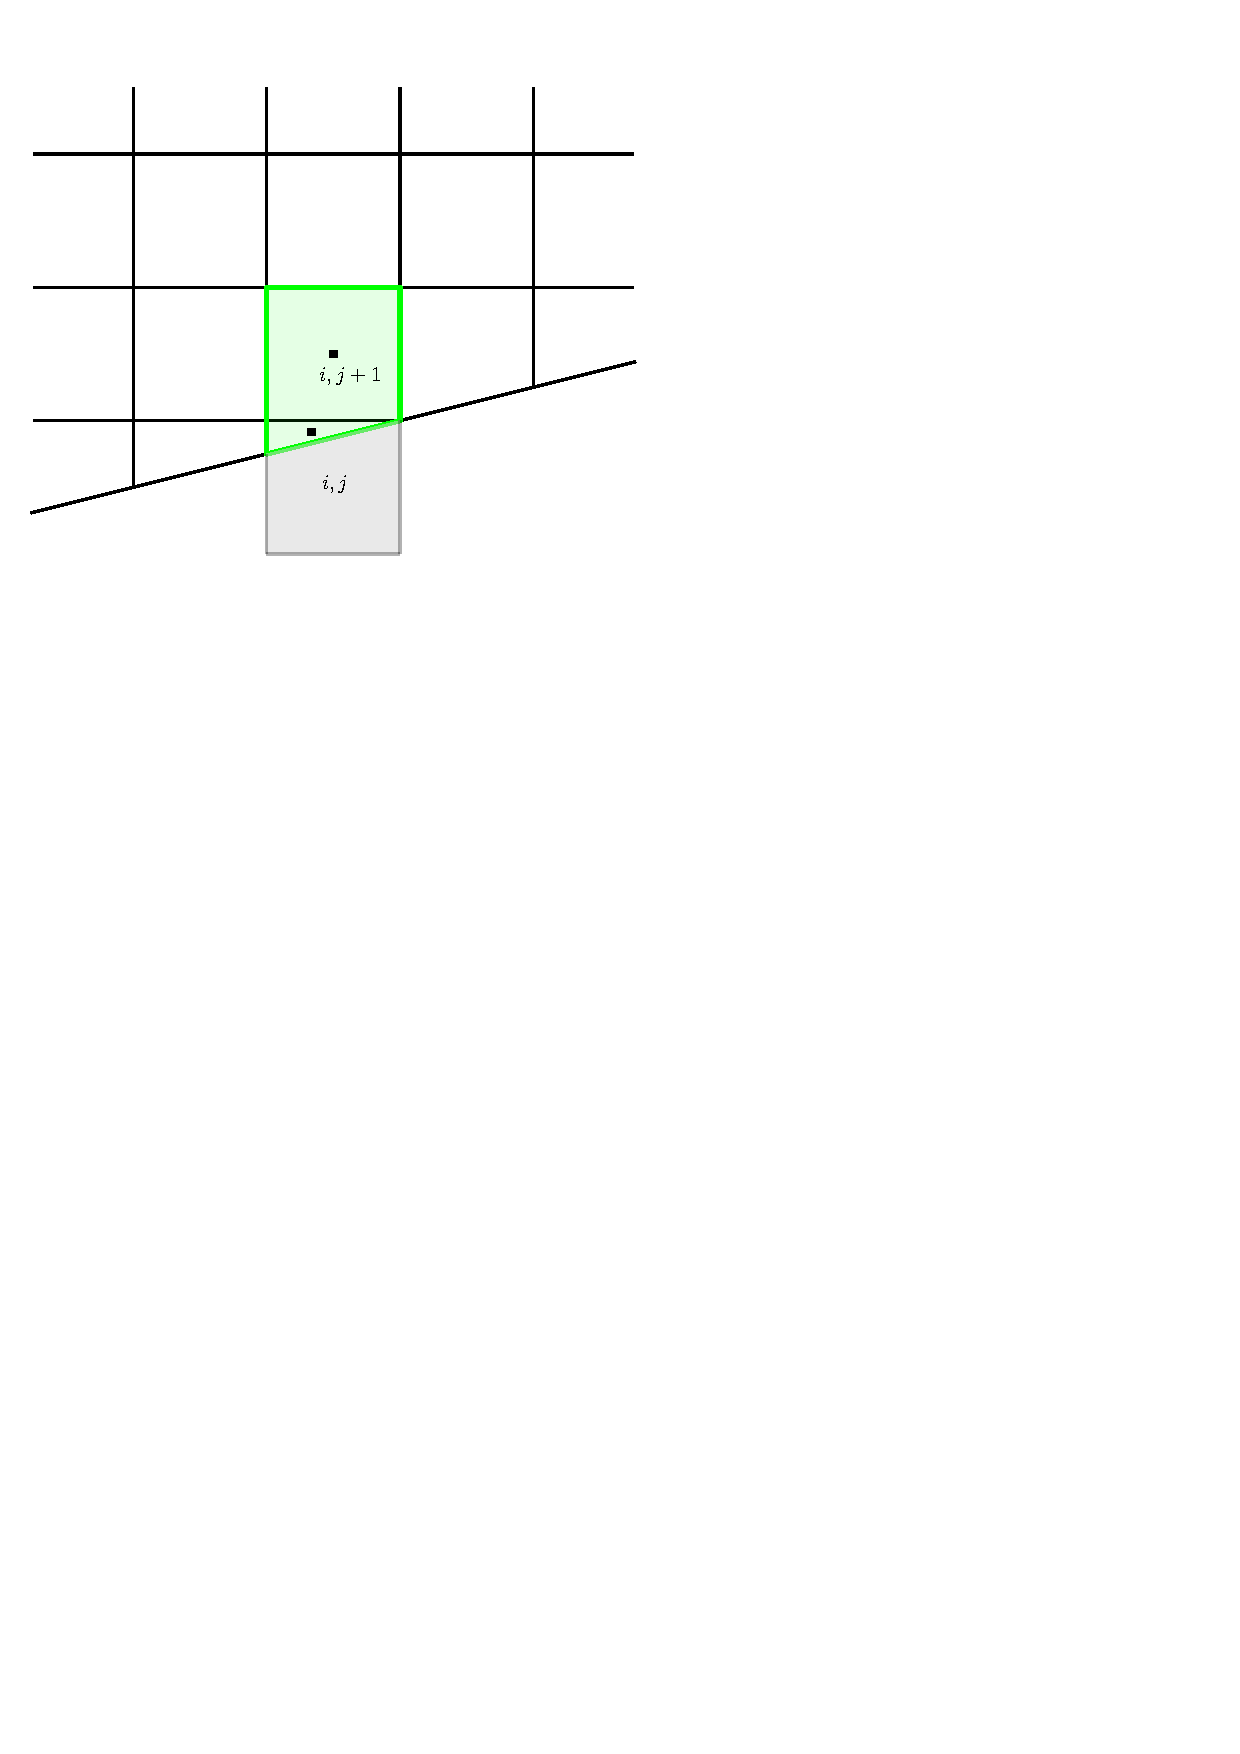
\includegraphics[width=.40\textwidth]{figs/modelexample2D_2.pdf} \label{fig:2nborTile2}}
	\caption{\sf Two-dimensional example of overlapping neighborhoods.  The unweighted centroids of cells $i,j$ and $i,j+1$ are indicated with solid squares ($\blacksquare$).} \label{fig:2nborTile}
\end{figure}

The conservation properties of the algorithm will be discussed after the
higher order SRD algorithm is presented in the next
section (PR PUT IT HERE). It will also be prseented more generally.   
OTHER THINGS HERE? DEMONSTRATE LINEARLY EXACT SECOND ORDER CONVERGENCE
HERE INSTEAD OF COMPRESULTS SECTION?

Different choices of neighborhoods, the minimum volume for the merging
neighborhood, gradient neighborhoods, and limiting will give
somewhat different computational results. Some of these will be examined
theoretically using model problems in one space dimension in section
\ref{sec:theory}. These choices can affect the stability limit of the
overall method.
We will also show computational results using different neighborhood
choices in section \ref{sec:compResults} in two space dimensions.

\subsection{Linear exactness}
In this section, we show that the SRD method preserves linear functions.  Consider the grid function of the numerical solution after one time step or stage, $\widehat{U}$.  Assume that it can be written in terms of a linear function $f(x,y)$ of the $x$ and $y$ coordinates, i.e.,
\begin{equation}
    \label{eqn:uhatlinear}
\widehat{U}_{i,j} = f(x_{i,j},y_{i,j}) = ax_{i,j} + by_{i,j} + c.
\end{equation}
From \eqref{eqn:uhatlinear} and the expression for the average on the merging neighborhood $i,j$, \eqref{tiledef}, we have
\begin{equation}
    \label{eqn:linear1}
\widehat{Q}_{i,j} = \frac{1}{{\widehat V}_{i,j}} \, \sum_{k \in M_i} \,  
\frac{V_k}{N_k}  \,\, (ax_{k} + by_{k} + c).
\end{equation}
Distributing the summation in \eqref{eqn:linear1}, we have
\begin{equation}\label{eqn:linear2}
\widehat{Q}_{i,j} =  a \left(\frac{1}{{\widehat V}_{i,j}} \, \sum_{k \in M_i} \,  
\frac{V_k}{N_k} x_{k} \right) + b\left(\frac{1}{{\widehat V}_{i,j}} \, \sum_{k \in M_i} \,  
\frac{V_k}{N_k} y_{k} \right) + c\left(\frac{1}{{\widehat V}_{i,j}} \, \sum_{k \in M_i} \,
\frac{V_k}{N_k}\right) .
\end{equation}
From the definition of the weighted centroid and volume of the merging neighborhood
$i,j$ in \eqref{voldef} and \eqref{centroiddef}, respectively, \eqref{eqn:linear2} becomes
\begin{equation}\label{eqn:linear3}
\widehat{Q}_{i,j} =  a \widehat{x}_{i,j} + b\widehat{y}_{i,j} + c = f(\widehat{x}_{i,j},\widehat{y}_{i,j}).
\end{equation}
Now, on the merging neighborhood $i,j$, we solve the least squares system in
\eqref{eqn:linrecon} to find $\widehat{\sigma}_{x,i,j}$ and
$\widehat{\sigma}_{y,i,j}$, i.e., the gradient on the merging neighborhood.  Using
\eqref{eqn:linear3} in \eqref{eqn:linrecon}, and due to the linearity of $f$, the following system
\begin{equation}
\widehat{\sigma}_{x,i,j}(\widehat{x}_{k} - \widehat{x}_{i,j}) + \widehat{\sigma}_{y,i,j}(\widehat{y}_{k} - \widehat{y}_{i,j})= f(\widehat{x}_k, \widehat{y}_k) - f(\widehat{x}_{i,j}, \widehat{y}_{i,j}) \quad \forall k \in R_{i,j},
\end{equation}
is solved exactly by $\widehat{\sigma}_{x,i,j}=a$ and
$\widehat{\sigma}_{y,i,j}=b$.  In other words, the exact gradient 
of $f$, $(a,b)$, is reconstructed on merging neighborhood $(i,j)$.  
The reconstructed solution is then
\begin{equation}
    \label{eqn:qrecon1}
    \hat{q}_{i,j}(x,y) = f(\widehat{x}_{i,j},\widehat{y}_{i,j}) + a(x-\widehat{x}_{i,j})+b(y-\widehat{y}_{i,j}) .
\end{equation}
Since $f$ is a linear function, \eqref{eqn:qrecon1} becomes
\begin{equation}
    \label{eqn:qrecon2}
    \hat{q}_{i,j}(x,y) = f(x,y).
\end{equation}
By \eqref{eqn:final_update_linear} and \eqref{eqn:qrecon2}, the final solution update is then
\begin{equation} 
U^{n+1}_{i,j} := \frac{1}{N_{i,j}}\sum_{k \in W_{i,j}}f(x_{i,j},y_{i,j}).
\end{equation}
This becomes
\begin{equation} 
U^{n+1}_{i,j} := f(x_{i,j},y_{i,j}),
\end{equation}
i.e., $U^{n+1}_{i,j} = \widehat{U}_{i,j}$, which shows that the SRD method is linearity preserving.

We conclude that the SRD algorithm will preserve the accuracy of a second order accurate 
base scheme. In section \ref{sec:ho} we will extend both SRD and the RK
schemes to third order or higher accuracy.

% The linear advection equation
% $$
% \begin{cases}
%  u_t + a u_x + b u_y = 0 \\
%  u(x,y,0) = f(x,y)
% \end{cases}
% $$
% has the exact solution $u(x,y,t) = f(x-at,y-bt)$.  
% The second order TVD Runge Kutta method stabilized by the SRD method is
% \begin{align}
% U^{(1)} &= ST(U^n + \Delta t L(U^n)),\\
% U^{(2)} &= ST(U^{(1)} + \Delta t L(U^{(1)})),\\
% U^{n+1} &= \frac{1}{2}(U^n + U^{(2)}).
% \end{align}
% The finite volume scheme on the cut cell grid is linearity preserving.  That is, if the initial condition $f$ is a linear function, then the intermediate solution $U^n + \Delta t L(U^n)$ is a grid function of the exact solution at the time $t^n + \Delta t$.  We now must show that the SRD method does not modify this intermediate solution.



%\subsection{Limiting}
%We design a linearity preserving scalar limiter for slopes on the merging neighborhoods.  
%Our goal is to limit the reconstructed gradient on merging neighborhood $i,j$.
%First, we compute the minimum and maximum merging neighborhood average over the reconstruction stencil $R_{i,j}$, i.e., 
%\begin{equation}
%     m_{i,j} = \max_{k \in R_{i,j}} \widehat{Q}_k \text{ and } M_{i,j} = \max_{k \in R_{i,j}} \widehat{Q}_k.
%\end{equation}
%The reconstructed gradient on merging neighborhood $i,j$ is limited by a nonnegative scalar $\alpha \in [0,1]$, i.e., the limited numerical solution on merging neighborhood $i,j$ is
%\begin{equation}
%    \tilde q_{i,j}(x,y) = \widehat{Q}_{i,j} + \alpha [\widehat{\sigma}_{x,i,j} ( x_{i,j} - \widehat x_{i,j}) \, 
%   + \widehat{\sigma}_{y,i,j}( y_{i,j} - \widehat y_{i,j})],
%\end{equation}
%where $\alpha$ reduces the gradient such that when $\widehat{q}_{i,j}$ is evaluated at the centroids of the neighborhoods in $R_{i,j}$ lies between $m_{i,j}$ and $M_{i,j}$.
%That is, $\alpha$ is given by
%$$
%\alpha = \max\left(0,\min_{k \in R_{i,j}} \alpha_k \right),
%$$
%with
%\begin{equation}
%    \alpha_k = \begin{cases}
%    \frac{\widehat{q}_{i,j}(\widehat x_{k}, \widehat y_{k}) - \widehat{Q}_{i,j}}{M_{i,j} - \widehat{Q}_{i,j}} \text{ if } \widehat{q}_{i,j}(\widehat x_{k}, \widehat y_{k}) - \widehat{Q}_{i,j} \geq 0,\\
%     \frac{\widehat{q}_{i,j}(\widehat x_{k}, \widehat y_{k}) - \widehat{Q}_{i,j}}{m_{i,j} - \widehat{Q}_{i,j}} \text{ if } \widehat{q}_{i,j}(\widehat x_{k}, \widehat y_{k}) - \widehat{Q}_{i,j} < 0.
%    \end{cases}
%\end{equation}
%With this limited gradient, the reconstruction on each merging neighborhood satisfies a local maximum principle
%$$
%m_{i,j} \leq \tilde{q}_{i,j}(\widehat x_k, \widehat y_k) \leq M_{i,j} ~ \forall k \in R_{i,j}.
%$$
%This limiter is linearity preserving since $\tilde{q}_{i,j}$ satisfies a local maximum principle at the points $(\widehat x_k, \widehat y_k) ~\forall k \in R_{i,j}$, which coincide with the points over which $m_{i,j}$ and $M_{i,j}$ are computed [cite lilia and mine JCP paper].
